\documentclass[thesis]{subfiles}

\begin{document}

\OnlyInSubfile{\setcounter{chapter}{1}}
\chapter{Macroscopic studies}
\label{sec:macroscopic}

\vskip2\baselineskip

A first way to approach the problem of coupled deformation and adsorption in
porous materials is through the use of macroscopic or thermodynamic modeling
methods. Such methods are based on classical thermodynamic principles and allow
us to a gain high-level understanding of the processes at play. In this section,
I will introduce the concept of thermodynamic potential and thermodynamic
ensemble, that can be used together to predict the evolution of a system. In a
second part, I will show how these potentials can be used to make predictions on
the co-adsorption of multiple gas in the same porous framework, but that one
needs to be careful to use the thermodynamic ensemble adapted to the problem at
hand.

\newpage
\section{Classical thermodynamics}
\subsection{First law of thermodynamics}

The starting point for the macroscopic methods I will describe here are the laws
of thermodynamics. The first law of thermodynamics is a generalization of the
conservation of energy during physical processes. It can be stated as follows:

\vskip0.8ex
\begin{quote}
    For a closed system, the change in energy between two states of internal
    thermodynamic equilibrium is the sum of the work of external forces and the
    heat received by the system.
\end{quote}
\vskip0.8ex

If we divide the total energy $E_\text{tot}$ of a system into its kinetic energy
$E_\text{kin}$, potential energy $E_\text{pot}$ and internal energy
$\mathcal{U}$, and letting $W$ be the work received by a system during a
transformation and $Q$ the heat transfer during the same transformation, the
first law of thermodynamics can be written as
\[\Delta E_\text{tot} = \Delta E_\text{kin} + \Delta E_\text{pot} + \Delta \mathcal{U} = W + Q.\]
If now we consider a system at rest in a constant external potential field,
$E_\text{kin}$ and $E_\text{pot}$ are constant, and we find the usual
formulation of the first law of thermodynamics:
\[\Delta \mathcal{U} = W + Q.\]
It is often interesting to use a differential formulation of this relation,
considering infinitesimal changes in $\mathcal{U}$, $W$, and $Q$:
\[\d \mathcal{U} = \delta Q + \delta W.\]
If the system composition is not constant, \ie if it is undergoing chemical
reactions or if the system is open and exchanges particles with an external
reservoir, we need to add another term depending on the quantity of matter
$\{n_i\}$ for each chemical specie in the system:
\[\d \mathcal{U} = \delta Q + \delta W - \sum_i \mu_i \d n_i.\label{eq:first-principle}\]
In this formulation, the $\mu_i$ are called the \emph{chemical potentials}; they
represent the relative stability of the different chemical species in the
system.

An interesting special case is that of an external pressure acting on the
system. In this case,
\[\delta W_\text{pressure} = -p_\text{ext} \d V \ ;\]
where $p_\text{ext}$ is the external pressure. If $p_\text{ext}$ is constant
during the transformation, this can be written as $\delta W_\text{pressure} =
-\d (PV)$, using $P$ as the constant value of the pressure. We can then define
the enthalpy $H$ as $H = \mathcal{U} + PV$ ; which allow us to rewrite
equation~\eqref{eq:first-principle} as
\[\d H = \delta Q + \delta W_\text{other} - \sum_i \mu_i \d n_i.\]
Here, $\delta W_\text{other}$ is the work coming from all forces
\emph{excluding} pressure forces.

\subsection{Second law of thermodynamics}

The second law of thermodynamics allows us to make predictions on the "natural"
evolution of a system.

\vskip0.8ex
\begin{quote}
    There exist a function of state called entropy, noted $S$, which is an
    increasing function of time for any transformation of an isolated system.
\end{quote}
\vskip0.8ex

The variation of entropy during a transformation of a closed system can be
linked to the heat transfer between the system and its surroundings by the
Clausius relation:
\[\Delta S = \frac Q T + S_\text{created}. \label{eq:clausius}\]
The $Q/T$ term is homogeneous to an entropy and called the exchanged entropy,
and is the entropy given to the system by its surroundings. $S_\text{created}$
is the entropy created during the transformation, and is a positive quantity by
the second law of thermodynamics. When $S_\text{created}$ is null, the
transformation is said to be \emph{reversible}.

Using the relations~\eqref{eq:first-principle} and~\eqref{eq:clausius}; and
considering that only the pressure forces act on the system, we can extract an
evolution principle for any transformation:
\[T \d S = \delta Q + \d S_\text{created}\]
\[T \d S = (\d \mathcal{U} - \delta W - \sum_i \mu_i \d n_i) + \d S_\text{created}\]
\[\d \mathcal{U} + P \d V  - \sum_i \mu_i \d n_i - T \d S = -T\delta S_\text{created}.\label{eq:thermo-potentials}\]
If there is a function $\Phi$ such as $\d \Phi = \d \mathcal{U} + P \d V - \sum_i \mu_i
n_i - T \d S$, then for any transformation of a closed system, $\d \Phi =
-T\delta S_\text{created} \leq 0$. This means that $\Phi$ is a decreasing
function of time, and it will be minimal in the equilibrium state. In this case,
$\Phi$ is called the \emph{thermodynamic potential}.

\subsection{Statistical ensembles}

A thermodynamic ensemble is defined by a set of thermodynamic state variable
that obey some constraints. For example the ensemble where the composition of
the system is fixed, together with the volume and total energy is called the
$NVE$ or micro-canonical ensemble. Other well known ensembles present a fixed
pressure or temperature: the $NVT$ or canonical ensemble, and the $NPT$ or
isobaric-isothermal ensemble.

Each of these ensembles has an associated thermodynamic potential. For the
micro-canonical ensemble, we start with equation~\eqref{eq:thermo-potentials}:
\[\d \Phi = \d \mathcal{U} + P \d V - \sum_i \mu_i \d n_i - T \d S.\]
$\d \mathcal{U}$ and $\d V$ will be zero as the energy and volume is constant.
Moreover as the system composition is fixed, $\d n_i = 0$. This gives
\[\d \Phi = - T \d S \leq 0.\]
The thermodynamic potential for the $NVE$ ensemble is the negentropy
$\mathcal{N} \equiv -TS$, which will be minimal (and the entropy will be
maximal) at equilibrium.

If we now allow the energy to change but fix the kinetic energy and thus the
temperature by the mean of an external thermostat,
equation~\eqref{eq:thermo-potentials} becomes
\[\d \Phi = \d \mathcal{U} + P \d V - \sum_i \mu_i \d n_i - T \d S - (S \d T - S \d T) \]
\[\d \Phi = \d \mathcal{U} + P \d V - \sum_i \mu_i \d n_i - \d (TS) + S \d T. \]
As the temperature, volume and composition are fixed, $\d T = \d V = \d n_i = 0$,
which means that
\[\d \Phi = \d (\mathcal{U} - TS).\]
We can introduce the Helmholtz free energy $F \equiv \mathcal{U} - TS$
(sometimes simply called free energy), which is the thermodynamic potential in
the $NVT$ ensemble.

If now we allow the volume to change in the system, while fixing the pressure
with a barostat and keeping the temperature fixed,
equation~\eqref{eq:thermo-potentials} becomes
\[\d \Phi = \d \mathcal{U} + P \d V + (V\d P - V\d P) - T \d S - (S\d T - S\d T) - \sum_i \mu_i \d n_i\]
\[\d \Phi = \d \mathcal{U} + \d (PV) - \d(TS) - V\d P + S\d T - \sum_i \mu_i \d n_i\]
Again, as the pressure, temperature and composition are fixed, this reduces to
\[\d \Phi = \d \mathcal{U} + \d (PV) - \d(TS).\]
We define the Gibbs free energy $G$ as $G \equiv \mathcal{U} + PV - TS \equiv F + PV
\equiv H - TS$, which is the thermodynamic potential in the $NPT$ ensemble.

\subsection{Ensembles for adsorption processes}
\label{sec:osmotic-ensemble}

Getting back to the topic of adsorption in porous material, we need to describe
the thermodynamic ensemble in which the adsorption process takes place. The
temperature is always fixed, as well as the composition of the adsorbing host.
If the host is rigid, and does not deform under adsorption, then we can consider
that the volume of the system is constant. The main difference with the
previously defined ensembles is that the composition of the gas phase is not
fixed: the number of gas molecules adsorbed in the system is allowed to change
during adsorption. In this case, equation~\eqref{eq:thermo-potentials} becomes
\[\d \Phi = \d \mathcal{U} - \d(TS) + P\d V + S\d T - \sum_i \mu_i \d n_i\]
Removing the null terms $\d V$ and $\d T$, we find the definition of the
\emph{grand-canonical} thermodynamic potential $\Psi$, associated with the
$\mu VT$ ensemble:
\[\Psi \equiv \mathcal{U} - TS - \sum_i \mu_i n_i \equiv F - \sum_i \mu_i n_i.\]
The Gibbs-Duhen relation ($V\d P - S\d T = \sum_i n_i \d\mu_i$) also gives us:
\[\Psi = -PV \]

If we now consider adsorption in a flexible host, the volume is no longer fixed.
Instead, in most experimental setups, external pressure is fixed and set equal
to the pressure of the adsorbed gases outside of the host. The thermodynamic
ensemble suited for the study of adsorption in flexible materials is called the
\emph{osmotic ensemble}, first introduced in 1994\cite{Mehta1994} for the study
of fluid mixtures, and adapted to multi-components phase equilibrium in
1998\cite{Escobedo1998}. Again, starting from equation~\eqref{eq:thermo-potentials}
\[\d \Phi = \d \mathcal{U} - \d (PV) - \d(TS) - V\d P + S\d T - \sum_i \mu_i \d n_i.\]
As usual, $\d T$ and $\d P$ are null as the corresponding variable is fixed. In
the sum over the $\mu_i n_i$ terms, only the adsorbed species quantities of
matter are allowed to change. The osmotic potential is thus defined by
\[\Omega \equiv \mathcal{U} - TS + PV - \sum_i \mu_i n_i \equiv F + PV - \sum_i \mu_i n_i \equiv G - \sum_i \mu_i n_i\]
This potential will be the basis we use to predict co-adsorption in flexible
porous media in the next section. The table~\ref{table:thermo-potential}
presents a summary of all the thermodynamic ensembles discussed so far, as well
as the associated fixed quantities and thermodynamic potentials.

\begin{table}[htp]
    \centering
    \renewcommand{\arraystretch}{1.3}
    \begin{tabularx}{0.8\textwidth}{l c c c X}
        Ensemble            & Fixed quantities                    & \multicolumn{3}{l}{Thermodynamic potential} \\ \hline
        Micro-canonical     & $N$, $V$, $E$                       & \hskip1em $\mathcal{N}$ & $\equiv$ & $-TS$                   \\
        Canonical           & $N$, $V$, $T$                       & \hskip1em $F$      & $\equiv$ & $\mathcal{U} - TS$      \\
        Isobaric-Isothermal & $N$, $P$, $T$                       & \hskip1em $G$      & $\equiv$ & $H - TS$                \\
        Grand-Canonical     & $\mu_i$, $V$, $T$                   & \hskip1em $\Psi$   & $\equiv$ & $F - \sum_i \mu_i n_i $ \\
        Osmotic             & $N_\text{host}$, $\mu_i$, $P$, $T$  & \hskip1em $\Omega$ & $\equiv$ & $G - \sum_i \mu_i n_i $ \\
    \end{tabularx}
    \caption{Thermodynamic ensembles and associated thermodynamic potentials}
    \label{table:thermo-potential}
\end{table}

\newpage
\section{Macroscopic calculations for gas separation in flexible materials}

Gas separation is an important step in multiple industrial processes, from
separation of hydrocarbons in oil chemistry, to \ce{CO2} separation and storage
or oxygen extraction in the air. The two main methods used for gas separation
are cryogenic distillation, mainly used for air separation, and differential
adsorption. Adsorption-based processes for gas separation, which rely on
microporous materials in the form of an adsorber bed, are very versatile because
of the large choice of materials available --- and the possibility to tune them
for a specific gas system. To choose an adsorber and the size of a production
plant for the separation of a gas mixture, good knowledge on the co-adsorption
of these gases in the candidate porous adsorbent is required.

Experimental characterization of this co-adsorption is typically done through
multi-component gas adsorption studies. This problem is inherently
high-dimensional, e.g., for a ternary mixture there are four variables to vary
(temperature, total pressure, and two independent variables for the mixture
composition). Because such experimental studies of co-adsorption equilibrium
thermodynamics are typically long and expensive, there has been a great expense
of literature devoted to theoretical models for the prediction of mixture
co-adsorption based on single-component adsorption data. The most commonly used
method in the field is the Ideal Adsorbed Solution Theory
(IAST)\cite{Myers1965}, which is relatively simple to implement and robust, and
allows the prediction of multi-component adsorption behavior from individual
single-component isotherms. Other theory are used when the ideality of the
system can no longer be assumed: non-ideal adsorbed solution
models\cite{Yang1987, Sweatman2002}, the vacancy solution theory
(VST)\cite{Suwanayuen1980}, the Real Adsorbed Solution Theory\cite{Talu1986}
(RAST), \etc

Materials which undergo large-scale reversible structural transitions impacting
their total volume or internal pore volume appear to be particular common among
metal-organic frameworks based on relatively weaker bonds (coordination bonds,
$\pi$--$\pi$ stacking, hydrogen bonds, or some covalent bonds) compared to
inorganic dense nanoporous materials (such as zeolites). In particular, some of
these materials show transitions between an \emph{open} phase with large pore
volume, and a \emph{condensed} or \emph{narrow pore} phase with smaller pore
volume --- or, in some cases, no microporosity at all. Such transitions, known
as \emph{gate opening}\cite{Kitaura2003, Tanaka2008, Li2015} or
\emph{breathing}\cite{Serre2002} depending on the order in which the phases
occur upon adsorption, can lead to stepped adsorption isotherms for pure
components.

In the recent literature, many authors have relied on IAST predictions to
predict that several such flexible MOFs would present very good selectivity for
gas separation. In some cases, the authors explicitly used IAST to derive such
predictions on flexible materials\cite{Banerjee2014, Mukherjee2015, Foo2016,
Li2016}. In other cases, IAST was not used explicitly, but the assumptions made
for the behavior of mixtures stem from the \emph{classical} understanding of
selectivity rules in rigid materials, and would not necessarily be valid in
flexible materials\cite{Gucuyener2010, Inubushi2010, Nijem2012, Sanda2013,
Joarder2014, Mukherjee2014}.

IAST is one of the available methods for direct macroscopic calculations and
predictions, taking macroscopic data in the form of pure component adsorption
isotherms and predicting macroscopic co-adsorption isotherms. In practice, using
IAST is akin to working in the Grand-Canonical ensemble, but we showed in the
previous section that when the adsorption host is flexible, one should use the
Osmotic ensemble. Instead, an alternative method called the Osmotic Framework
Adsorbed Solution Theory (OFAST)\cite{Coudert2009}, based on the Osmotic
ensemble, should be used when structural transitions occur during adsorption.
This theory has been developed in the group\cite{Coudert2010,Ortiz2011}, and
takes into account the coupling between adsorption and deformations in flexible
porous materials.

% For example \citeauthor{Nijem2012} \cite{Nijem2012} reported
% that \emph{"[their] work unveils unexpected hydrocarbon selectivity in a
% flexible metal-organic framework (MOF), based on differences in their gate
% opening pressure."}

In this section, I will compare the results of IAST and OFAST on two sets of
adsorption data from the published literature on gate-opening materials, and
show that the IAST method gives unrealistic results: it does not reproduce the
gate-opening behavior upon mixture adsorption, and overestimates the selectivity
by up to two orders of magnitude. All of this work is published in
\citejournal{Fraux2018}\cite{Fraux2018}.

\subsection{Ideal Adsorbed Solution Theory}

The Ideal Adsorbed Solution Theory (IAST) starts by assuming that for a given
adsorbent and at fixed temperature $T$, the pure-component isotherms $n_i(P)$
for each gas $i$ of interest is known. Then, given a mixture of ideal gases
adsorbing at total pressure $P$ in an host framework and the composition of the
gas phase $y_i$ --- such that the partial pressures follow the ideal mixing law
$P_i = y_i P$ --- the goal of the method is to predict the total adsorbed
quantity $n_\text{tot}$ and the molar fractions $x_i$ in the adsorbed phase.

In order to do so, \citeauthor{Myers1965}\cite{Myers1965} introduced for each
mixture component a quantity homogeneous to a pressure, $P_i^*$. The IAST method
links this pressure to the compositions of the gas and adsorbed phases by
defining a link between $P_i^*$ and the known variables:
\[P y_i = P_i^* x_i ;\label{eq:spreading}\]
and by imposing the equality of chemical potentials at thermodynamic equilibrium:
\[\label{eq:chem-pot} \forall i,j \quad \int_0^{P_i^*} \frac{n_i(p)}{p} \d p = \int_0^{P_j^*} \frac{n_j(p)}{p} \d p .\]

In the simpler case of two-component gas mixture containing gases B and C, these
two equations and the conservation of matter can be rewritten as a set of four
equations:
\[\begin{gathered}
    P y_B = P_B^* x_B \kern10em x_B = \frac{P_C^* - P}{P_C^* - P_B^*} \\[0.5em]
    \frac1{n_\text{tot}} = \frac{x_B}{n_B(P_B^*)} + \frac{1 - x_B}{n_C(P_C^*)} \\[1.2em]
    \label{eq:iast}\int_0^{P_B^*} \frac{n_B(p)}{p} \d p = \int_0^{P_C^*} \frac{n_C(p)}{p} \d p
\end{gathered}\]

Solving these equations for $P_B^*$ and $P_C^*$ will give all the information on
the system composition. It can be done with either numerical integration of the
isotherms, or by fitting the isotherms to a model, and then integrating the
model analytically.

\newpage
\subsection{IAST and flexible frameworks}

The original derivation of the IAST equations\cite{Myers1965} by
\citeauthor{Myers1965} highlights three hypotheses on the co-adsorption process,
on which the model is built:
\begin{description}
    \item[(H1)] The adsorbing framework is inert from a thermodynamic point of view;
    \item[(H2)] The adsorbing framework specific area is constant with respect to
                temperature and the same for all adsorbed species;
    \item[(H3)] The Gibbs definition of adsorption applies.
\end{description}

While the meaning of the last assumption \textbf{(H3)} has been diversely
interpreted by different authors, Myers\cite{Myers1965} originally meant and
later confirmed\cite{Myers2014} it to qualify the method by which the adsorption
isotherms are measured. There is, however, consensus on the fact that absolute
adsorption should be used in IAST calculations --- as opposed to excess or net
adsorption\cite{Brandani2016}. This assumption thus applies equally to both
rigid and flexible adsorbents. However, the first two hypothesis are not valid
for flexible nanoporous materials. \textbf{(H2)} is clearly invalid, as
modifications in both the host's volume and internal structure lead to
variations of pore size and specific area upon structural transitions. We note
here, in passing, that \textbf{(H2)} should already be ruled out for systems of
pore size close to the adsorbate diameter, as well as gas mixtures of widely
different size or shape.  It should, for example, not apply to molecular sieves
systems, yet those can often be described reasonably well by IAST in practice.
Finally, \textbf{(H1)} is violated by all the systems that feature
adsorption-induced deformation, and in particular by systems presenting a
gate-opening or a breathing behavior. As a conclusion, IAST has no theoretical
foundation for those systems and should not be used for co-adsorption prediction
in flexible nanoporous frameworks.

\begin{figure}[htp]
    \centering
    % GNUPLOT: LaTeX picture with Postscript
\begingroup
  \makeatletter
  \providecommand\color[2][]{%
    \GenericError{(gnuplot) \space\space\space\@spaces}{%
      Package color not loaded in conjunction with
      terminal option `colourtext'%
    }{See the gnuplot documentation for explanation.%
    }{Either use 'blacktext' in gnuplot or load the package
      color.sty in LaTeX.}%
    \renewcommand\color[2][]{}%
  }%
  \providecommand\includegraphics[2][]{%
    \GenericError{(gnuplot) \space\space\space\@spaces}{%
      Package graphicx or graphics not loaded%
    }{See the gnuplot documentation for explanation.%
    }{The gnuplot epslatex terminal needs graphicx.sty or graphics.sty.}%
    \renewcommand\includegraphics[2][]{}%
  }%
  \providecommand\rotatebox[2]{#2}%
  \@ifundefined{ifGPcolor}{%
    \newif\ifGPcolor
    \GPcolortrue
  }{}%
  \@ifundefined{ifGPblacktext}{%
    \newif\ifGPblacktext
    \GPblacktextfalse
  }{}%
  % define a \g@addto@macro without @ in the name:
  \let\gplgaddtomacro\g@addto@macro
  % define empty templates for all commands taking text:
  \gdef\gplbacktext{}%
  \gdef\gplfronttext{}%
  \makeatother
  \ifGPblacktext
    % no textcolor at all
    \def\colorrgb#1{}%
    \def\colorgray#1{}%
  \else
    % gray or color?
    \ifGPcolor
      \def\colorrgb#1{\color[rgb]{#1}}%
      \def\colorgray#1{\color[gray]{#1}}%
      \expandafter\def\csname LTw\endcsname{\color{white}}%
      \expandafter\def\csname LTb\endcsname{\color{black}}%
      \expandafter\def\csname LTa\endcsname{\color{black}}%
      \expandafter\def\csname LT0\endcsname{\color[rgb]{1,0,0}}%
      \expandafter\def\csname LT1\endcsname{\color[rgb]{0,1,0}}%
      \expandafter\def\csname LT2\endcsname{\color[rgb]{0,0,1}}%
      \expandafter\def\csname LT3\endcsname{\color[rgb]{1,0,1}}%
      \expandafter\def\csname LT4\endcsname{\color[rgb]{0,1,1}}%
      \expandafter\def\csname LT5\endcsname{\color[rgb]{1,1,0}}%
      \expandafter\def\csname LT6\endcsname{\color[rgb]{0,0,0}}%
      \expandafter\def\csname LT7\endcsname{\color[rgb]{1,0.3,0}}%
      \expandafter\def\csname LT8\endcsname{\color[rgb]{0.5,0.5,0.5}}%
    \else
      % gray
      \def\colorrgb#1{\color{black}}%
      \def\colorgray#1{\color[gray]{#1}}%
      \expandafter\def\csname LTw\endcsname{\color{white}}%
      \expandafter\def\csname LTb\endcsname{\color{black}}%
      \expandafter\def\csname LTa\endcsname{\color{black}}%
      \expandafter\def\csname LT0\endcsname{\color{black}}%
      \expandafter\def\csname LT1\endcsname{\color{black}}%
      \expandafter\def\csname LT2\endcsname{\color{black}}%
      \expandafter\def\csname LT3\endcsname{\color{black}}%
      \expandafter\def\csname LT4\endcsname{\color{black}}%
      \expandafter\def\csname LT5\endcsname{\color{black}}%
      \expandafter\def\csname LT6\endcsname{\color{black}}%
      \expandafter\def\csname LT7\endcsname{\color{black}}%
      \expandafter\def\csname LT8\endcsname{\color{black}}%
    \fi
  \fi
    \setlength{\unitlength}{0.0500bp}%
    \ifx\gptboxheight\undefined%
      \newlength{\gptboxheight}%
      \newlength{\gptboxwidth}%
      \newsavebox{\gptboxtext}%
    \fi%
    \setlength{\fboxrule}{0.5pt}%
    \setlength{\fboxsep}{1pt}%
\begin{picture}(4520.00,2820.00)%
    \gplgaddtomacro\gplbacktext{%
    }%
    \gplgaddtomacro\gplfronttext{%
      \csname LTb\endcsname%%
      \put(153,1474){\rotatebox{-270}{\makebox(0,0){\strut{}uptake}}}%
      \csname LTb\endcsname%%
      \put(2271,130){\makebox(0,0){\strut{}pressure}}%
      \colorrgb{0.90,0.12,0.06}%%
      \put(395,2001){\makebox(0,0)[l]{\strut{}closed}}%
      \colorrgb{0.90,0.12,0.06}%%
      \put(1689,2001){\makebox(0,0)[l]{\strut{}open}}%
      \colorrgb{0.00,0.45,0.70}%%
      \put(1301,737){\makebox(0,0)[l]{\strut{}closed}}%
      \colorrgb{0.00,0.45,0.70}%%
      \put(2595,737){\makebox(0,0)[l]{\strut{}open}}%
      \csname LTb\endcsname%%
      \put(3339,2106){\makebox(0,0)[l]{\strut{}$\Delta n$}}%
    }%
    \gplbacktext
    \put(0,0){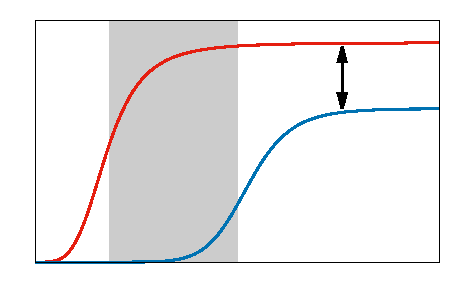
\includegraphics{open-close-selectivity}}%
    \gplfronttext
  \end{picture}%
\endgroup

    \caption{Typical single-component isotherms for adsorption of two gases (red
    and blue) in a material with gate opening. The gate opening pressure is not
    the same for the two adsorbates, creating a pressure range with a high
    difference in the adsorption capacity for single-components isotherms (gray
    zone in the figure). Contrary to intuition, selectivity will not necessarily
    by high in this pressure range, but will depend on difference in saturation
    uptake $\Delta n$.}
    \label{fig:open-close-selectivity}
\end{figure}

Aside from the mathematical treatment and thermodynamic hypotheses, we can show
in an qualitative way why it is not possible, in flexible host frameworks, to
use the single-component isotherm directly to predict multi-components
adsorption. We address here a common misconception, due to an invalid graphical
interpretation of the isotherms. Figure~\ref{fig:open-close-selectivity} depicts
the equilibrium adsorption isotherms for two different guests in a material
presenting a gate-opening behavior. The gate opening is an adsorption-induced
structural transition from a nonporous to a porous phase of the host, leading to
a step in the single-component adsorption isotherm. Gate opening occurs at two
different pressures for the two adsorbates, due to the specific host--guest
interactions of the two gases (characterized notably by the enthalpy of
adsorption and saturation uptake). In the pressure range in-between the
transition pressures (in gray in figure~\ref{fig:open-close-selectivity}), the
uptake of one species is close to zero --- \emph{in the single-component
isotherm} --- and the uptake of the other species is close to its maximum value.
If these isotherms were encountered for a rigid host material, the selectivity
would be extremely high in this range, with one guest adsorbing but not the
other.

Yet, the step in the isotherms here is not simply linked to host--guest
interactions but indeed due to a change in the host structure. In particular,
upon adsorption of a gas mixture in this gate-opening framework, a phase
transition will occur at a given pressure. Before this transition, the structure
will be contracted and show no (or little) adsorption for either guest, and thus
no usable selectivity. After the transition, \emph{both species} will adsorb
into the open pore framework. The selectivity is then governed --- at least
qualitatively --- by the respective saturation uptakes of the two fluids
($\Delta n$ in the figure). While the difference in adsorbed quantities in the
intermediate pressure range visually suggests great selectivity, it is not
possible for one component to adsorb inside the close phase framework while at
the same time the other component adsorbs inside the open phase of the framework.
The framework is either in one phase or in the other, at any given time.

\begin{figure}[htp]
    \centering
    % GNUPLOT: LaTeX picture with Postscript
\begingroup
  \makeatletter
  \providecommand\color[2][]{%
    \GenericError{(gnuplot) \space\space\space\@spaces}{%
      Package color not loaded in conjunction with
      terminal option `colourtext'%
    }{See the gnuplot documentation for explanation.%
    }{Either use 'blacktext' in gnuplot or load the package
      color.sty in LaTeX.}%
    \renewcommand\color[2][]{}%
  }%
  \providecommand\includegraphics[2][]{%
    \GenericError{(gnuplot) \space\space\space\@spaces}{%
      Package graphicx or graphics not loaded%
    }{See the gnuplot documentation for explanation.%
    }{The gnuplot epslatex terminal needs graphicx.sty or graphics.sty.}%
    \renewcommand\includegraphics[2][]{}%
  }%
  \providecommand\rotatebox[2]{#2}%
  \@ifundefined{ifGPcolor}{%
    \newif\ifGPcolor
    \GPcolortrue
  }{}%
  \@ifundefined{ifGPblacktext}{%
    \newif\ifGPblacktext
    \GPblacktextfalse
  }{}%
  % define a \g@addto@macro without @ in the name:
  \let\gplgaddtomacro\g@addto@macro
  % define empty templates for all commands taking text:
  \gdef\gplbacktext{}%
  \gdef\gplfronttext{}%
  \makeatother
  \ifGPblacktext
    % no textcolor at all
    \def\colorrgb#1{}%
    \def\colorgray#1{}%
  \else
    % gray or color?
    \ifGPcolor
      \def\colorrgb#1{\color[rgb]{#1}}%
      \def\colorgray#1{\color[gray]{#1}}%
      \expandafter\def\csname LTw\endcsname{\color{white}}%
      \expandafter\def\csname LTb\endcsname{\color{black}}%
      \expandafter\def\csname LTa\endcsname{\color{black}}%
      \expandafter\def\csname LT0\endcsname{\color[rgb]{1,0,0}}%
      \expandafter\def\csname LT1\endcsname{\color[rgb]{0,1,0}}%
      \expandafter\def\csname LT2\endcsname{\color[rgb]{0,0,1}}%
      \expandafter\def\csname LT3\endcsname{\color[rgb]{1,0,1}}%
      \expandafter\def\csname LT4\endcsname{\color[rgb]{0,1,1}}%
      \expandafter\def\csname LT5\endcsname{\color[rgb]{1,1,0}}%
      \expandafter\def\csname LT6\endcsname{\color[rgb]{0,0,0}}%
      \expandafter\def\csname LT7\endcsname{\color[rgb]{1,0.3,0}}%
      \expandafter\def\csname LT8\endcsname{\color[rgb]{0.5,0.5,0.5}}%
    \else
      % gray
      \def\colorrgb#1{\color{black}}%
      \def\colorgray#1{\color[gray]{#1}}%
      \expandafter\def\csname LTw\endcsname{\color{white}}%
      \expandafter\def\csname LTb\endcsname{\color{black}}%
      \expandafter\def\csname LTa\endcsname{\color{black}}%
      \expandafter\def\csname LT0\endcsname{\color{black}}%
      \expandafter\def\csname LT1\endcsname{\color{black}}%
      \expandafter\def\csname LT2\endcsname{\color{black}}%
      \expandafter\def\csname LT3\endcsname{\color{black}}%
      \expandafter\def\csname LT4\endcsname{\color{black}}%
      \expandafter\def\csname LT5\endcsname{\color{black}}%
      \expandafter\def\csname LT6\endcsname{\color{black}}%
      \expandafter\def\csname LT7\endcsname{\color{black}}%
      \expandafter\def\csname LT8\endcsname{\color{black}}%
    \fi
  \fi
    \setlength{\unitlength}{0.0500bp}%
    \ifx\gptboxheight\undefined%
      \newlength{\gptboxheight}%
      \newlength{\gptboxwidth}%
      \newsavebox{\gptboxtext}%
    \fi%
    \setlength{\fboxrule}{0.5pt}%
    \setlength{\fboxsep}{1pt}%
\begin{picture}(4520.00,2820.00)%
    \gplgaddtomacro\gplbacktext{%
      \csname LTb\endcsname%%
      \put(1550,1475){\makebox(0,0)[l]{\strut{}$P_\text{trans}$}}%
    }%
    \gplgaddtomacro\gplfronttext{%
      \csname LTb\endcsname%%
      \put(153,1474){\rotatebox{-270}{\makebox(0,0){\strut{}uptake}}}%
      \csname LTb\endcsname%%
      \put(2271,130){\makebox(0,0){\strut{}pressure}}%
      \csname LTb\endcsname%%
      \put(3425,1715){\makebox(0,0)[r]{\strut{}flexible}}%
      \csname LTb\endcsname%%
      \put(3425,1474){\makebox(0,0)[r]{\strut{}open}}%
      \csname LTb\endcsname%%
      \put(3425,1233){\makebox(0,0)[r]{\strut{}closed}}%
    }%
    \gplbacktext
    \put(0,0){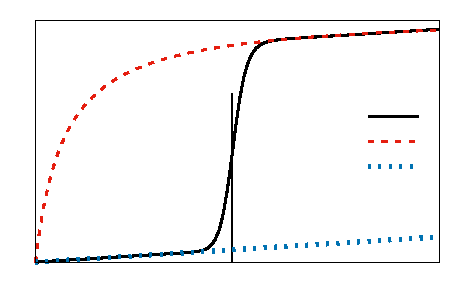
\includegraphics{open-close-isotherms}}%
    \gplfronttext
  \end{picture}%
\endgroup

    \caption{Generation of the total isotherm in gate-opening materials by the
    combination of two single-phase isotherms: an \emph{open} pores isotherm,
    and an \emph{closed} pores isotherm. The transition between the two host
    phases occurs at $P_\text{trans}$.}
    \label{fig:open-close-isotherms}
\end{figure}

The whole issue with using single-component isotherms to predict multi-component
adsorption in frameworks with phase transition boils down to the origin of the
stepped isotherms. The single-component isotherm (represented in
figure~\ref{fig:open-close-isotherms}) is a combination of two isotherms: one in
the first phase (the contracted pore phase), and one in the second phase (the
open pore phase). Both phases --- and the thermodynamic equilibrium between them
--- need to be taken in account to predict the multi-component adsorption.

\subsection{Osmotic Framework Adsorbed Solution Theory}

As established in section~\ref{sec:osmotic-ensemble}, the thermodynamic ensemble
suited for the study of adsorption in flexible materials is the osmotic
ensemble. Let's recall that in this ensemble, the thermodynamic potential
$\Omega$ is a function of the mechanical pressure $P$, the temperature $T$, the
number of atoms in a given host phase $\alpha$ and the adsorbed species chemical
potentials $\mu_i$:
\[\Omega(T, P, \mu_i) = F_\alpha + P V_\alpha - \sum_i \mu_i n_{\alpha,i},\]
where $F_\alpha$ is the Helmholtz free energy of the empty host in phase
$\alpha$, $V_\alpha$ the volume of the host in this phase, and $n_{\alpha,i}$
the molar uptake of guest $i$ in phase $\alpha$. This expression can be reworked
and expressed as a function not of chemical potentials, but of fluid pressure
(taken equal to mechanical pressure $P$) and adsorption
isotherms:\cite{Coudert2008}
\[ \label{eq:osmotic-potential}\Omega(T, P, \mu_i) = F_\alpha + P V_\alpha - \sum_i \int_0^P n_{\alpha,i}(T, p) V^m_i(T, p) \ \d p\]
Here, $n_{\alpha,i}(T,P)$ are the co-adsorption isotherms for each component and
$V^m_i(T,P)$ the molar volume for the species $i$ in the bulk phase. Supposing
that the gases are ideal, the molar volume is given by $RT/P$, with $R$ the
ideal gas constant.

I have shown previously that IAST cannot be used for the study of co-adsorption
in frameworks with adsorption-induced phases transition, because the framework
is not inert during adsorption. However, the IAST assumptions are still valid
for each individual phase of the host matrix, if they are considered in the
absence of a transition. As a consequence, it means that the IAST model can be
used, for each possible host phase $\alpha$, to calculate the co-adsorption
isotherms $n_{\alpha,i}(P,T)$ in this given phase. Then, the thermodynamic
potential of each phase $\Omega_{\alpha}$ can be calculated from these isotherms
through Equation~\eqref{eq:osmotic-potential}, allowing to predict which phase
is the more stable at a given gas phase pressure and composition --- and where
the structural transition(s) occur. This method, extending the IAST theory in
the osmotic ensemble to account for host flexibility, has been called Osmotic
Framework Adsorbed Solution Theory (OFAST)\cite{Coudert2009, Coudert2010}.

Although the amount of published data from direct experimental measurements of
co-adsorption of gas mixtures in flexible MOFs is very limited, the OFAST method
has been well validated in the past against experimental data.\cite{Ortiz2011,
Hoffmann2011, Zang2011}. For example, \citeauthor{Ortiz2011}\cite{Ortiz2011}
compared the method against experimental data for adsorption of
\ce{CO2}/\ce{CH4} mixtures in the MIL-53(Al) MOF. MIL-53(Al) is the seminal
example of material with a \emph{breathing} behavior: at low loadings, its most
stable phase is the high porous volume \emph{open-pore} phases, at intermediate
loadings it transition to a \emph{closed-pore} phase, and at high loading it
goes back to the open-pore structure. One of the very interesting things that
\citeauthor{Ortiz2011} predicted using OFAST is the increase of the stability
domain of the closed pore phase when using mixtures with respect to pure
component adsorption. The predicted phase diagrams of MIL-53(Al) is reproduced
in figure~\ref{fig:ofast:ortiz}.

\begin{figure}[ht]
    \centering
    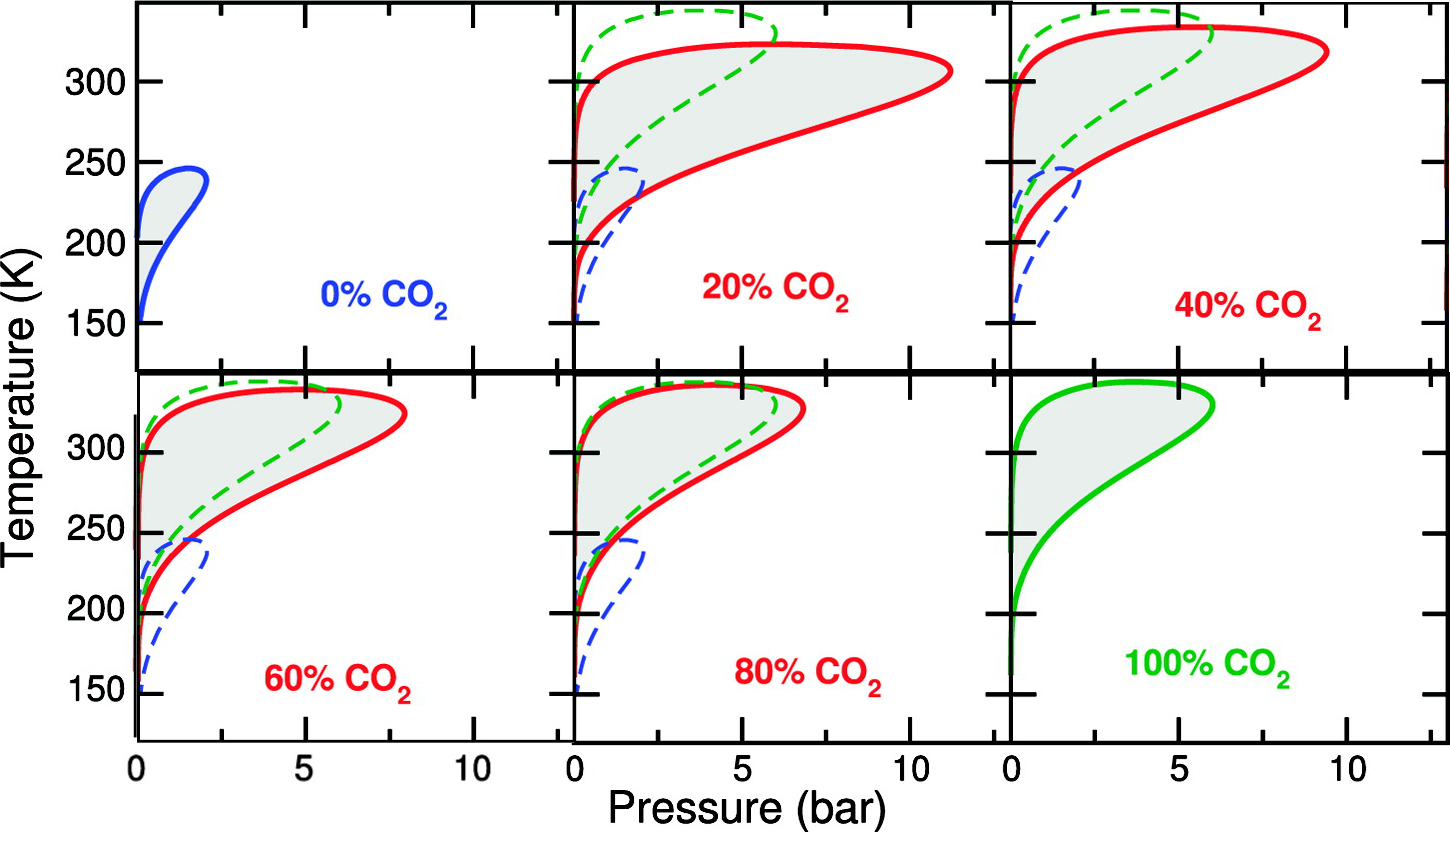
\includegraphics[width=0.8\textwidth]{figures/cited/ofast-phase-diagram-rotated}
    \caption{Temperature–pressure phase diagram of MIL-53(Al) upon adsorption
    of a \ce{CO2}/\ce{CH4} mixture, with increasing \ce{CO2} molar fraction.
    Dashed lines correspond to pure component diagrams.
    Reproduced from reference~\cite{Ortiz2011}.}
    \label{fig:ofast:ortiz}
\end{figure}

In practice, the use of OFAST follows the following steps. First, the host
phases of interest are identified and the single-component adsorption isotherms
$n_{\alpha,i}(T, p)$ for these are obtained: this can be achieved from a fit of
experimental isotherms (see figure~\ref{fig:open-close-isotherms}) or from
molecular simulation.

Secondly, the relative free energies of the host phases (which reduces to a
single $\Delta F_\text{host}$ in our case of two host phases) can be computed
from equation~\eqref{eq:osmotic-potential} and the experimental single-component
stepped isotherm. For example, with two phases $\alpha$ and $\beta$, and
considering ideal gas, we can express equation~\eqref{eq:osmotic-potential} for
each phase:
\[\Omega_\alpha(T, P, \mu_i) = F_\alpha + P V_\alpha - RT \sum_i \int_0^P \frac{n_{\alpha, i}(p)}{p} \ \d p\]
\[\Omega_\beta(T, P, \mu_i) = F_\beta + P V_\beta - RT \sum_i \int_0^P \frac{n_{\beta, i}(p)}{p} \ \d p\]
At the transition ($P=P_\text{trans}$ in figure~\ref{fig:open-close-isotherms},
which is typically known experimentally) the two thermodynamic potentials will
be equal, which gives us a way to evaluate the free energy difference between
the phases:
\[ \label{eq:ofast:delta-f}\Delta F_\text{host} = RT \sum_i \int_0^{P_\text{trans}} \frac{\Delta n_i(T, p)}{p} \d p - P_\text{trans} \Delta V_\text{host}\]

Then, for all values of thermodynamic parameters of interest (pressure and gas
mixture composition) the osmotic potential of the host phases is computed,
enabling the identification of the most stable phase: the phase with the lowest
osmotic potential is the most stable at this pressure and composition. The
pressures at which the osmotic potential in both phases are equal are the phase
transition pressures for a given composition. Finally, we can compute adsorption
properties (guest uptake and selectivity) using IAST in each phase, within its
domain of stability.

\newpage
\subsection{Comparing IAST and OFAST}

I present here two examples of co-adsorption of gas mixtures in metal-organic
frameworks with gate opening behavior, based on experimental data from the
published literature, comparing the predictions of IAST with those of OFAST. The
first example deals with the adsorption of $\ce{CO2}$, $\ce{CH4}$, and $\ce{O2}$
in the \Cudhbc MOF\cite{Kitaura2003} (see figure~\ref{fig:cu-dhbc}; dhbc =
2,5-dihydroxybenzoate; bpy = bipyridine). These isotherms correspond very
closely to the archetypal \emph{gate opening} scenario described above. The
second example deals with linear alkanes (ethane, propane, and butane)
adsorption in \RPMZn MOF\cite{Nijem2012}; figure~\ref{fig:rpm3-zn} presents the
framework structure of \RPMZn and relevant experimental adsorption and
desorption isotherms.

\subsubsection{Simple isotherms in \Cudhbc}

\begin{figure}[htp]
    \centering
    \raisebox{-0.5\height}{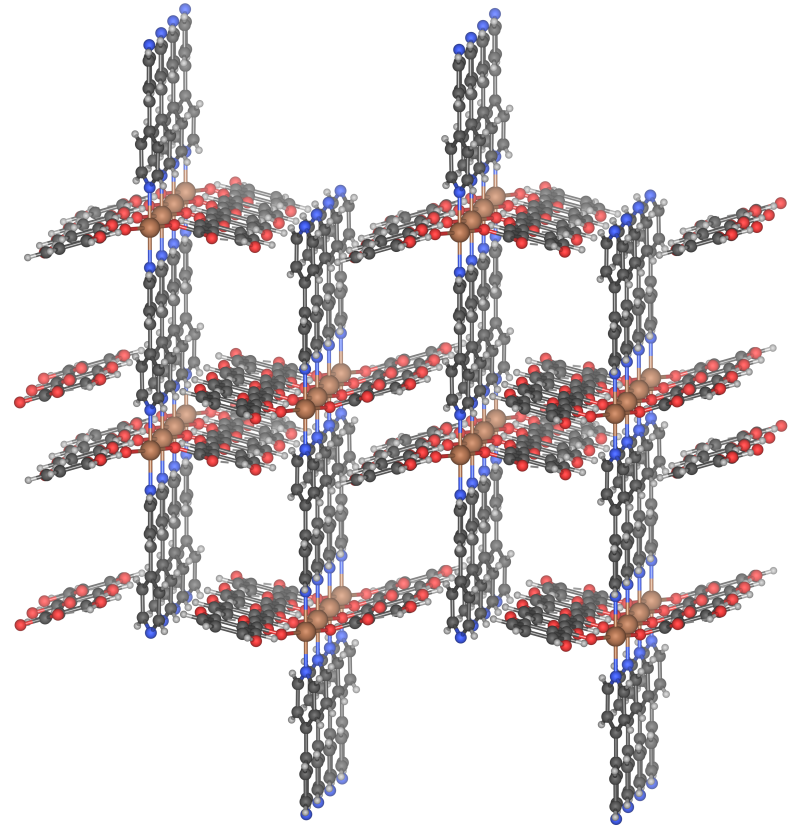
\includegraphics[width=0.35\textwidth]{figures/images/cu-dhbc-structure}}
    \hfill
    \raisebox{-0.5\height}{% GNUPLOT: LaTeX picture with Postscript
\begingroup
  \makeatletter
  \providecommand\color[2][]{%
    \GenericError{(gnuplot) \space\space\space\@spaces}{%
      Package color not loaded in conjunction with
      terminal option `colourtext'%
    }{See the gnuplot documentation for explanation.%
    }{Either use 'blacktext' in gnuplot or load the package
      color.sty in LaTeX.}%
    \renewcommand\color[2][]{}%
  }%
  \providecommand\includegraphics[2][]{%
    \GenericError{(gnuplot) \space\space\space\@spaces}{%
      Package graphicx or graphics not loaded%
    }{See the gnuplot documentation for explanation.%
    }{The gnuplot epslatex terminal needs graphicx.sty or graphics.sty.}%
    \renewcommand\includegraphics[2][]{}%
  }%
  \providecommand\rotatebox[2]{#2}%
  \@ifundefined{ifGPcolor}{%
    \newif\ifGPcolor
    \GPcolortrue
  }{}%
  \@ifundefined{ifGPblacktext}{%
    \newif\ifGPblacktext
    \GPblacktextfalse
  }{}%
  % define a \g@addto@macro without @ in the name:
  \let\gplgaddtomacro\g@addto@macro
  % define empty templates for all commands taking text:
  \gdef\gplbacktext{}%
  \gdef\gplfronttext{}%
  \makeatother
  \ifGPblacktext
    % no textcolor at all
    \def\colorrgb#1{}%
    \def\colorgray#1{}%
  \else
    % gray or color?
    \ifGPcolor
      \def\colorrgb#1{\color[rgb]{#1}}%
      \def\colorgray#1{\color[gray]{#1}}%
      \expandafter\def\csname LTw\endcsname{\color{white}}%
      \expandafter\def\csname LTb\endcsname{\color{black}}%
      \expandafter\def\csname LTa\endcsname{\color{black}}%
      \expandafter\def\csname LT0\endcsname{\color[rgb]{1,0,0}}%
      \expandafter\def\csname LT1\endcsname{\color[rgb]{0,1,0}}%
      \expandafter\def\csname LT2\endcsname{\color[rgb]{0,0,1}}%
      \expandafter\def\csname LT3\endcsname{\color[rgb]{1,0,1}}%
      \expandafter\def\csname LT4\endcsname{\color[rgb]{0,1,1}}%
      \expandafter\def\csname LT5\endcsname{\color[rgb]{1,1,0}}%
      \expandafter\def\csname LT6\endcsname{\color[rgb]{0,0,0}}%
      \expandafter\def\csname LT7\endcsname{\color[rgb]{1,0.3,0}}%
      \expandafter\def\csname LT8\endcsname{\color[rgb]{0.5,0.5,0.5}}%
    \else
      % gray
      \def\colorrgb#1{\color{black}}%
      \def\colorgray#1{\color[gray]{#1}}%
      \expandafter\def\csname LTw\endcsname{\color{white}}%
      \expandafter\def\csname LTb\endcsname{\color{black}}%
      \expandafter\def\csname LTa\endcsname{\color{black}}%
      \expandafter\def\csname LT0\endcsname{\color{black}}%
      \expandafter\def\csname LT1\endcsname{\color{black}}%
      \expandafter\def\csname LT2\endcsname{\color{black}}%
      \expandafter\def\csname LT3\endcsname{\color{black}}%
      \expandafter\def\csname LT4\endcsname{\color{black}}%
      \expandafter\def\csname LT5\endcsname{\color{black}}%
      \expandafter\def\csname LT6\endcsname{\color{black}}%
      \expandafter\def\csname LT7\endcsname{\color{black}}%
      \expandafter\def\csname LT8\endcsname{\color{black}}%
    \fi
  \fi
    \setlength{\unitlength}{0.0500bp}%
    \ifx\gptboxheight\undefined%
      \newlength{\gptboxheight}%
      \newlength{\gptboxwidth}%
      \newsavebox{\gptboxtext}%
    \fi%
    \setlength{\fboxrule}{0.5pt}%
    \setlength{\fboxsep}{1pt}%
\begin{picture}(4520.00,3400.00)%
    \gplgaddtomacro\gplbacktext{%
      \csname LTb\endcsname%%
      \put(441,595){\makebox(0,0)[r]{\strut{}$0$}}%
      \csname LTb\endcsname%%
      \put(441,1468){\makebox(0,0)[r]{\strut{}$1$}}%
      \csname LTb\endcsname%%
      \put(441,2340){\makebox(0,0)[r]{\strut{}$2$}}%
      \csname LTb\endcsname%%
      \put(441,3213){\makebox(0,0)[r]{\strut{}$3$}}%
      \csname LTb\endcsname%%
      \put(543,409){\makebox(0,0){\strut{}$0$}}%
      \csname LTb\endcsname%%
      \put(1461,409){\makebox(0,0){\strut{}$20$}}%
      \csname LTb\endcsname%%
      \put(2378,409){\makebox(0,0){\strut{}$40$}}%
      \csname LTb\endcsname%%
      \put(3296,409){\makebox(0,0){\strut{}$60$}}%
      \csname LTb\endcsname%%
      \put(4213,409){\makebox(0,0){\strut{}$80$}}%
    }%
    \gplgaddtomacro\gplfronttext{%
      \csname LTb\endcsname%%
      \put(153,1904){\rotatebox{-270}{\makebox(0,0){\strut{}uptake / (mol/mol)}}}%
      \csname LTb\endcsname%%
      \put(2378,130){\makebox(0,0){\strut{}pressure / atm}}%
      \csname LTb\endcsname%%
      \put(3425,1271){\makebox(0,0)[r]{\strut{}CH$_4$}}%
      \csname LTb\endcsname%%
      \put(3425,1030){\makebox(0,0)[r]{\strut{}CO$_2$}}%
      \csname LTb\endcsname%%
      \put(3425,789){\makebox(0,0)[r]{\strut{}O$_2$}}%
    }%
    \gplbacktext
    \put(0,0){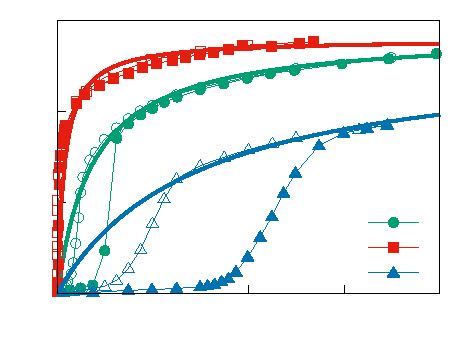
\includegraphics{cu-dhbc}}%
    \gplfronttext
  \end{picture}%
\endgroup
}
    \caption{(left) \Cudhbc structure (from reference.~\cite{Kitaura2003}). (right)
    Sorption isotherms and model isotherms fit at \SI{298}{K} in \Cudhbc for
    various gas compounds. Adsorption data are presented using filled symbols,
    and desorption data using empty symbols. Thick lines are Langmuir isotherms
    fitted at high loading. Experimental data published by
    \citeauthor{Kitaura2003}\cite{Kitaura2003}}
    \label{fig:cu-dhbc}
\end{figure}

\Cudhbc is a textbook example of gate opening upon adsorption, with
single-component adsorption isotherms (reproduced in figure~\ref{fig:cu-dhbc})
that clearly show the transition from a nonporous (at low gas pressure) to a
microporous (at higher pressure) host phase. From the experimental
data\cite{Kitaura2003} I fitted the isotherms at high loading using a Langmuir
model (equation~\eqref{eq:langmuir-isotherm}) for the isotherm in the open-pore
structure; and at low loading using a Henry isotherm model
(equation~\eqref{eq:henry-isotherm}) for the closed-pore structure following the
model proposed in figure~\ref{fig:open-close-isotherms}. Langmuir model is able
to reproduce type I isotherms, and Henry model is usually valid for low
loadings.
\[N(p) = K_H \ p \label{eq:henry-isotherm}\]
\[N(p) = N_L \ \frac{K_L \ p}{1 + K_L \ p} \label{eq:langmuir-isotherm}\]

\begin{table}[htp]
    \centering
    \renewcommand{\arraystretch}{1.2}
    \newcolumntype{C}{>{\centering\arraybackslash}X}
    \begin{tabularx}{\textwidth}{c C c C c C}
        \textbf{Gas} & $K_H$ / (mol/atm) & $N_L$ / mol & $K_L$ / atm & $P_\text{trans}$ / atm & $\Delta F$ / (kJ/mol)  \\ \hline
        \ce{CH4}     &     0.0           & 2.86      & 0.134         &                5       & -3.56                  \\
        \ce{CO2}     &     0.0           & 2.79      & 0.699         &                1       & -3.59                  \\
        \ce{O2}      &     0.0           & 2.68      & 0.034         &               20       & -3.39                  \\
    \end{tabularx}
    \caption{Fitted coefficients for the sorption isotherms and free energy
    difference between open and closed structures in \Cudhbc. See
    equations~\eqref{eq:henry-isotherm} and \eqref{eq:langmuir-isotherm} for the
    definitions of $K_H$, $N_L$ and $K_L$.}
    \label{table:cu-dhbc:fit}
\end{table}

The resulting fit parameters are in table~\ref{table:cu-dhbc:fit}. In the
closed-pore phase, I assumed that no adsorption takes place in the whole
pressure range, this is why the $K_H$ coefficient is always zero. Using these
parameters and equation~\eqref{eq:ofast:delta-f}, I computed the free energy
difference for all the isotherms. I took the value of $-3.5 \pm
\SI{0.1}{kJ/mol}$ as the free energy difference between the phases.

I performed OFAST calculations using Wolfram Mathematica, the corresponding code
is available in the lab's GitHub repository\cite{fx-citable-data}. I used the
PyIAST Python package for the  pure IAST calculations\cite{Simon2016}. For these
IAST calculations, I did not fit the isotherms to a specific model, but rather
solved the IAST equations by numerical integration and interpolation between
experimental data points. At partial pressures higher than the last point in the
experimental isotherm, that last point was used as saturation uptake. I computed
both partial loading and selectivity between the different gas in a mixture.

Figure~\ref{fig:cu-dhbc:iast-ofast:selectivity} presents the selectivity
obtained with IAST and OFAST; and figure~\ref{fig:cu-dhbc:iast-ofast:loadings}
shows the partial and total loadings for all the gas combinations. The
adsorption selectivity calculated with OFAST follows what one would expect: at
low pressure, the pores are closed and no gas enter the structure, making the
selectivity ill-defined --- the isotherms at low pressure cannot be fitted and
exploited for calculation of separation.  Then, at a pressure depending on the
composition of the gas phase, the gate opening transition occurs. At pressure
higher than gate opening pressure, the framework is in its open pore form, and
the value of selectivity depends on the relative saturation uptake of the two
phases. The selectivities observed are almost independent of the fluid mixture
composition, they are~$\approx 20$ for \ce{CO2}/\ce{O2} and~$\approx 4$ for
\ce{CH4}/\ce{O2} mixtures.

\begin{figure}[htp]
    \centering
    % GNUPLOT: LaTeX picture with Postscript
\begingroup
  \makeatletter
  \providecommand\color[2][]{%
    \GenericError{(gnuplot) \space\space\space\@spaces}{%
      Package color not loaded in conjunction with
      terminal option `colourtext'%
    }{See the gnuplot documentation for explanation.%
    }{Either use 'blacktext' in gnuplot or load the package
      color.sty in LaTeX.}%
    \renewcommand\color[2][]{}%
  }%
  \providecommand\includegraphics[2][]{%
    \GenericError{(gnuplot) \space\space\space\@spaces}{%
      Package graphicx or graphics not loaded%
    }{See the gnuplot documentation for explanation.%
    }{The gnuplot epslatex terminal needs graphicx.sty or graphics.sty.}%
    \renewcommand\includegraphics[2][]{}%
  }%
  \providecommand\rotatebox[2]{#2}%
  \@ifundefined{ifGPcolor}{%
    \newif\ifGPcolor
    \GPcolortrue
  }{}%
  \@ifundefined{ifGPblacktext}{%
    \newif\ifGPblacktext
    \GPblacktextfalse
  }{}%
  % define a \g@addto@macro without @ in the name:
  \let\gplgaddtomacro\g@addto@macro
  % define empty templates for all commands taking text:
  \gdef\gplbacktext{}%
  \gdef\gplfronttext{}%
  \makeatother
  \ifGPblacktext
    % no textcolor at all
    \def\colorrgb#1{}%
    \def\colorgray#1{}%
  \else
    % gray or color?
    \ifGPcolor
      \def\colorrgb#1{\color[rgb]{#1}}%
      \def\colorgray#1{\color[gray]{#1}}%
      \expandafter\def\csname LTw\endcsname{\color{white}}%
      \expandafter\def\csname LTb\endcsname{\color{black}}%
      \expandafter\def\csname LTa\endcsname{\color{black}}%
      \expandafter\def\csname LT0\endcsname{\color[rgb]{1,0,0}}%
      \expandafter\def\csname LT1\endcsname{\color[rgb]{0,1,0}}%
      \expandafter\def\csname LT2\endcsname{\color[rgb]{0,0,1}}%
      \expandafter\def\csname LT3\endcsname{\color[rgb]{1,0,1}}%
      \expandafter\def\csname LT4\endcsname{\color[rgb]{0,1,1}}%
      \expandafter\def\csname LT5\endcsname{\color[rgb]{1,1,0}}%
      \expandafter\def\csname LT6\endcsname{\color[rgb]{0,0,0}}%
      \expandafter\def\csname LT7\endcsname{\color[rgb]{1,0.3,0}}%
      \expandafter\def\csname LT8\endcsname{\color[rgb]{0.5,0.5,0.5}}%
    \else
      % gray
      \def\colorrgb#1{\color{black}}%
      \def\colorgray#1{\color[gray]{#1}}%
      \expandafter\def\csname LTw\endcsname{\color{white}}%
      \expandafter\def\csname LTb\endcsname{\color{black}}%
      \expandafter\def\csname LTa\endcsname{\color{black}}%
      \expandafter\def\csname LT0\endcsname{\color{black}}%
      \expandafter\def\csname LT1\endcsname{\color{black}}%
      \expandafter\def\csname LT2\endcsname{\color{black}}%
      \expandafter\def\csname LT3\endcsname{\color{black}}%
      \expandafter\def\csname LT4\endcsname{\color{black}}%
      \expandafter\def\csname LT5\endcsname{\color{black}}%
      \expandafter\def\csname LT6\endcsname{\color{black}}%
      \expandafter\def\csname LT7\endcsname{\color{black}}%
      \expandafter\def\csname LT8\endcsname{\color{black}}%
    \fi
  \fi
    \setlength{\unitlength}{0.0500bp}%
    \ifx\gptboxheight\undefined%
      \newlength{\gptboxheight}%
      \newlength{\gptboxwidth}%
      \newsavebox{\gptboxtext}%
    \fi%
    \setlength{\fboxrule}{0.5pt}%
    \setlength{\fboxsep}{1pt}%
\begin{picture}(7360.00,6800.00)%
    \gplgaddtomacro\gplbacktext{%
      \csname LTb\endcsname%%
      \put(747,4971){\makebox(0,0)[r]{\strut{}$0$}}%
      \csname LTb\endcsname%%
      \put(747,5628){\makebox(0,0)[r]{\strut{}$1000$}}%
      \csname LTb\endcsname%%
      \put(747,6285){\makebox(0,0)[r]{\strut{}$2000$}}%
      \csname LTb\endcsname%%
      \put(849,4719){\makebox(0,0){\strut{}$0$}}%
      \csname LTb\endcsname%%
      \put(1480,4719){\makebox(0,0){\strut{}$20$}}%
      \csname LTb\endcsname%%
      \put(2111,4719){\makebox(0,0){\strut{}$40$}}%
      \csname LTb\endcsname%%
      \put(2742,4719){\makebox(0,0){\strut{}$60$}}%
      \csname LTb\endcsname%%
      \put(3373,4719){\makebox(0,0){\strut{}$80$}}%
    }%
    \gplgaddtomacro\gplfronttext{%
      \csname LTb\endcsname%%
      \put(153,5759){\rotatebox{-270}{\makebox(0,0){\strut{}\ce{CO2} / \ce{O2} selectivity}}}%
      \csname LTb\endcsname%%
      \put(2585,6418){\makebox(0,0)[r]{\strut{}$y_{\ce{CO2}} = 0.1$}}%
      \csname LTb\endcsname%%
      \put(2585,6177){\makebox(0,0)[r]{\strut{}$y_{\ce{CO2}} = 0.5$}}%
      \csname LTb\endcsname%%
      \put(2585,5936){\makebox(0,0)[r]{\strut{}$y_{\ce{CO2}} = 0.9$}}%
    }%
    \gplgaddtomacro\gplbacktext{%
      \csname LTb\endcsname%%
      \put(4241,4905){\makebox(0,0)[r]{\strut{}$1$}}%
      \csname LTb\endcsname%%
      \put(4241,5343){\makebox(0,0)[r]{\strut{}$10$}}%
      \csname LTb\endcsname%%
      \put(4241,5780){\makebox(0,0)[r]{\strut{}$100$}}%
      \csname LTb\endcsname%%
      \put(4241,6218){\makebox(0,0)[r]{\strut{}$1000$}}%
      \csname LTb\endcsname%%
      \put(4343,4719){\makebox(0,0){\strut{}$0$}}%
      \csname LTb\endcsname%%
      \put(5021,4719){\makebox(0,0){\strut{}$20$}}%
      \csname LTb\endcsname%%
      \put(5698,4719){\makebox(0,0){\strut{}$40$}}%
      \csname LTb\endcsname%%
      \put(6376,4719){\makebox(0,0){\strut{}$60$}}%
      \csname LTb\endcsname%%
      \put(7053,4719){\makebox(0,0){\strut{}$80$}}%
    }%
    \gplgaddtomacro\gplfronttext{%
    }%
    \gplgaddtomacro\gplbacktext{%
      \csname LTb\endcsname%%
      \put(543,2719){\makebox(0,0)[r]{\strut{}$0$}}%
      \csname LTb\endcsname%%
      \put(543,3533){\makebox(0,0)[r]{\strut{}$5$}}%
      \csname LTb\endcsname%%
      \put(543,4347){\makebox(0,0)[r]{\strut{}$10$}}%
      \csname LTb\endcsname%%
      \put(645,2452){\makebox(0,0){\strut{}$0$}}%
      \csname LTb\endcsname%%
      \put(1327,2452){\makebox(0,0){\strut{}$20$}}%
      \csname LTb\endcsname%%
      \put(2009,2452){\makebox(0,0){\strut{}$40$}}%
      \csname LTb\endcsname%%
      \put(2691,2452){\makebox(0,0){\strut{}$60$}}%
      \csname LTb\endcsname%%
      \put(3373,2452){\makebox(0,0){\strut{}$80$}}%
    }%
    \gplgaddtomacro\gplfronttext{%
      \csname LTb\endcsname%%
      \put(153,3492){\rotatebox{-270}{\makebox(0,0){\strut{}\ce{CH4} / \ce{O2} selectivity}}}%
    }%
    \gplgaddtomacro\gplbacktext{%
      \csname LTb\endcsname%%
      \put(4037,2638){\makebox(0,0)[r]{\strut{}$1$}}%
      \csname LTb\endcsname%%
      \put(4037,4347){\makebox(0,0)[r]{\strut{}$10$}}%
      \csname LTb\endcsname%%
      \put(4139,2452){\makebox(0,0){\strut{}$0$}}%
      \csname LTb\endcsname%%
      \put(4868,2452){\makebox(0,0){\strut{}$20$}}%
      \csname LTb\endcsname%%
      \put(5596,2452){\makebox(0,0){\strut{}$40$}}%
      \csname LTb\endcsname%%
      \put(6325,2452){\makebox(0,0){\strut{}$60$}}%
      \csname LTb\endcsname%%
      \put(7053,2452){\makebox(0,0){\strut{}$80$}}%
    }%
    \gplgaddtomacro\gplfronttext{%
    }%
    \gplgaddtomacro\gplbacktext{%
      \csname LTb\endcsname%%
      \put(645,595){\makebox(0,0)[r]{\strut{}$0$}}%
      \csname LTb\endcsname%%
      \put(645,1338){\makebox(0,0)[r]{\strut{}$0.5$}}%
      \csname LTb\endcsname%%
      \put(645,2080){\makebox(0,0)[r]{\strut{}$1$}}%
      \csname LTb\endcsname%%
      \put(747,409){\makebox(0,0){\strut{}$0$}}%
      \csname LTb\endcsname%%
      \put(1404,409){\makebox(0,0){\strut{}$20$}}%
      \csname LTb\endcsname%%
      \put(2060,409){\makebox(0,0){\strut{}$40$}}%
      \csname LTb\endcsname%%
      \put(2717,409){\makebox(0,0){\strut{}$60$}}%
      \csname LTb\endcsname%%
      \put(3373,409){\makebox(0,0){\strut{}$80$}}%
    }%
    \gplgaddtomacro\gplfronttext{%
      \csname LTb\endcsname%%
      \put(153,1337){\rotatebox{-270}{\makebox(0,0){\strut{}\ce{CH4} / \ce{CO2} selectivity}}}%
      \csname LTb\endcsname%%
      \put(2060,130){\makebox(0,0){\strut{}pressure / atm}}%
    }%
    \gplgaddtomacro\gplbacktext{%
      \csname LTb\endcsname%%
      \put(4241,595){\makebox(0,0)[r]{\strut{}$0.01$}}%
      \csname LTb\endcsname%%
      \put(4241,1338){\makebox(0,0)[r]{\strut{}$0.1$}}%
      \csname LTb\endcsname%%
      \put(4241,2080){\makebox(0,0)[r]{\strut{}$1$}}%
      \csname LTb\endcsname%%
      \put(4343,409){\makebox(0,0){\strut{}$0$}}%
      \csname LTb\endcsname%%
      \put(5021,409){\makebox(0,0){\strut{}$20$}}%
      \csname LTb\endcsname%%
      \put(5698,409){\makebox(0,0){\strut{}$40$}}%
      \csname LTb\endcsname%%
      \put(6376,409){\makebox(0,0){\strut{}$60$}}%
      \csname LTb\endcsname%%
      \put(7053,409){\makebox(0,0){\strut{}$80$}}%
    }%
    \gplgaddtomacro\gplfronttext{%
      \csname LTb\endcsname%%
      \put(5698,130){\makebox(0,0){\strut{}pressure / atm}}%
    }%
    \gplbacktext
    \put(0,0){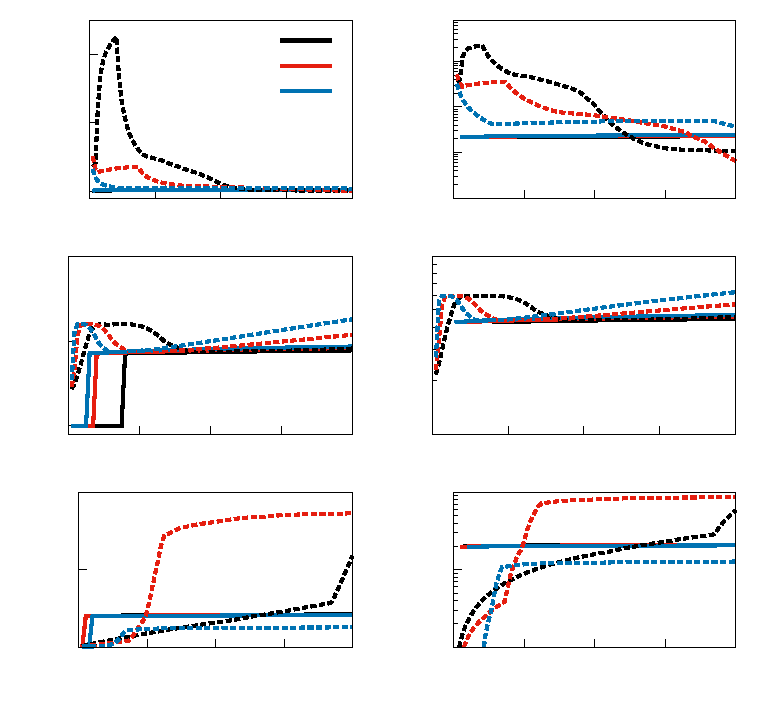
\includegraphics{cu-dhbc-selectivities}}%
    \gplfronttext
  \end{picture}%
\endgroup

    \caption{Comparison of IAST (dashed lines) and OFAST (plain lines)
    adsorption selectivity for \ce{CO2}/\ce{O2} (top); \ce{CH4}/\ce{O2} (middle)
    and \ce{CH4}/\ce{CO2} (bottom) mixtures in \Cudhbc. The same curves are
    presented twice, using linear scale for the $y$ axis on the left panels, and
    logarithmic scale on the right panels.}
    \label{fig:cu-dhbc:iast-ofast:selectivity}
\end{figure}

\begin{figure}[htp]
    \centering
    % GNUPLOT: LaTeX picture with Postscript
\begingroup
  \makeatletter
  \providecommand\color[2][]{%
    \GenericError{(gnuplot) \space\space\space\@spaces}{%
      Package color not loaded in conjunction with
      terminal option `colourtext'%
    }{See the gnuplot documentation for explanation.%
    }{Either use 'blacktext' in gnuplot or load the package
      color.sty in LaTeX.}%
    \renewcommand\color[2][]{}%
  }%
  \providecommand\includegraphics[2][]{%
    \GenericError{(gnuplot) \space\space\space\@spaces}{%
      Package graphicx or graphics not loaded%
    }{See the gnuplot documentation for explanation.%
    }{The gnuplot epslatex terminal needs graphicx.sty or graphics.sty.}%
    \renewcommand\includegraphics[2][]{}%
  }%
  \providecommand\rotatebox[2]{#2}%
  \@ifundefined{ifGPcolor}{%
    \newif\ifGPcolor
    \GPcolortrue
  }{}%
  \@ifundefined{ifGPblacktext}{%
    \newif\ifGPblacktext
    \GPblacktextfalse
  }{}%
  % define a \g@addto@macro without @ in the name:
  \let\gplgaddtomacro\g@addto@macro
  % define empty templates for all commands taking text:
  \gdef\gplbacktext{}%
  \gdef\gplfronttext{}%
  \makeatother
  \ifGPblacktext
    % no textcolor at all
    \def\colorrgb#1{}%
    \def\colorgray#1{}%
  \else
    % gray or color?
    \ifGPcolor
      \def\colorrgb#1{\color[rgb]{#1}}%
      \def\colorgray#1{\color[gray]{#1}}%
      \expandafter\def\csname LTw\endcsname{\color{white}}%
      \expandafter\def\csname LTb\endcsname{\color{black}}%
      \expandafter\def\csname LTa\endcsname{\color{black}}%
      \expandafter\def\csname LT0\endcsname{\color[rgb]{1,0,0}}%
      \expandafter\def\csname LT1\endcsname{\color[rgb]{0,1,0}}%
      \expandafter\def\csname LT2\endcsname{\color[rgb]{0,0,1}}%
      \expandafter\def\csname LT3\endcsname{\color[rgb]{1,0,1}}%
      \expandafter\def\csname LT4\endcsname{\color[rgb]{0,1,1}}%
      \expandafter\def\csname LT5\endcsname{\color[rgb]{1,1,0}}%
      \expandafter\def\csname LT6\endcsname{\color[rgb]{0,0,0}}%
      \expandafter\def\csname LT7\endcsname{\color[rgb]{1,0.3,0}}%
      \expandafter\def\csname LT8\endcsname{\color[rgb]{0.5,0.5,0.5}}%
    \else
      % gray
      \def\colorrgb#1{\color{black}}%
      \def\colorgray#1{\color[gray]{#1}}%
      \expandafter\def\csname LTw\endcsname{\color{white}}%
      \expandafter\def\csname LTb\endcsname{\color{black}}%
      \expandafter\def\csname LTa\endcsname{\color{black}}%
      \expandafter\def\csname LT0\endcsname{\color{black}}%
      \expandafter\def\csname LT1\endcsname{\color{black}}%
      \expandafter\def\csname LT2\endcsname{\color{black}}%
      \expandafter\def\csname LT3\endcsname{\color{black}}%
      \expandafter\def\csname LT4\endcsname{\color{black}}%
      \expandafter\def\csname LT5\endcsname{\color{black}}%
      \expandafter\def\csname LT6\endcsname{\color{black}}%
      \expandafter\def\csname LT7\endcsname{\color{black}}%
      \expandafter\def\csname LT8\endcsname{\color{black}}%
    \fi
  \fi
    \setlength{\unitlength}{0.0500bp}%
    \ifx\gptboxheight\undefined%
      \newlength{\gptboxheight}%
      \newlength{\gptboxwidth}%
      \newsavebox{\gptboxtext}%
    \fi%
    \setlength{\fboxrule}{0.5pt}%
    \setlength{\fboxsep}{1pt}%
\begin{picture}(7580.00,9060.00)%
    \gplgaddtomacro\gplbacktext{%
      \csname LTb\endcsname%%
      \put(860,6354){\makebox(0,0)[r]{\strut{}\small 0}}%
      \csname LTb\endcsname%%
      \put(860,6981){\makebox(0,0)[r]{\strut{}\small 1}}%
      \csname LTb\endcsname%%
      \put(860,7607){\makebox(0,0)[r]{\strut{}\small 2}}%
      \csname LTb\endcsname%%
      \put(860,8234){\makebox(0,0)[r]{\strut{}\small 3}}%
      \csname LTb\endcsname%%
      \put(962,6168){\makebox(0,0){\strut{}\small 0}}%
      \csname LTb\endcsname%%
      \put(1669,6168){\makebox(0,0){\strut{}\small 20}}%
      \csname LTb\endcsname%%
      \put(2376,6168){\makebox(0,0){\strut{}\small 40}}%
      \csname LTb\endcsname%%
      \put(3082,6168){\makebox(0,0){\strut{}\small 60}}%
      \csname LTb\endcsname%%
      \put(3789,6168){\makebox(0,0){\strut{}\small 80}}%
      \csname LTb\endcsname%%
      \put(1971,8878){\makebox(0,0)[l]{\strut{}OFAST}}%
      \csname LTb\endcsname%%
      \put(5457,8878){\makebox(0,0)[l]{\strut{}IAST}}%
      \csname LTb\endcsname%%
      \put(152,6794){\rotatebox{-270}{\makebox(0,0)[l]{\strut{}\ce{CO2} / \ce{O2}}}}%
      \csname LTb\endcsname%%
      \put(152,4348){\rotatebox{-270}{\makebox(0,0)[l]{\strut{}\ce{CH4} / \ce{O2}}}}%
      \csname LTb\endcsname%%
      \put(152,1268){\rotatebox{-270}{\makebox(0,0)[l]{\strut{}\ce{CH4} / \ce{CO2}}}}%
    }%
    \gplgaddtomacro\gplfronttext{%
      \csname LTb\endcsname%%
      \put(572,7294){\rotatebox{-270}{\makebox(0,0){\strut{}uptake / (mol/mol)}}}%
      \colorrgb{0.58,0.00,0.83}%%
      \put(1899,8487){\makebox(0,0)[r]{\strut{}\footnotesize $y_\smallce{CO2} \kern-0.5ex= 0.1$}}%
      \colorrgb{0.00,0.62,0.45}%%
      \put(2715,8487){\makebox(0,0)[r]{\strut{}\footnotesize ~~$y_\smallce{CO2} \kern-0.5ex= 0.5$}}%
      \colorrgb{0.00,0.45,0.70}%%
      \put(3531,8487){\makebox(0,0)[r]{\strut{}\footnotesize ~~$y_\smallce{CO2} \kern-0.5ex= 0.9$}}%
    }%
    \gplgaddtomacro\gplbacktext{%
      \csname LTb\endcsname%%
      \put(4271,6354){\makebox(0,0)[r]{\strut{}\small 0}}%
      \csname LTb\endcsname%%
      \put(4271,6981){\makebox(0,0)[r]{\strut{}\small 1}}%
      \csname LTb\endcsname%%
      \put(4271,7607){\makebox(0,0)[r]{\strut{}\small 2}}%
      \csname LTb\endcsname%%
      \put(4271,8234){\makebox(0,0)[r]{\strut{}\small 3}}%
      \csname LTb\endcsname%%
      \put(4373,6168){\makebox(0,0){\strut{}\small 0}}%
      \csname LTb\endcsname%%
      \put(5080,6168){\makebox(0,0){\strut{}\small 20}}%
      \csname LTb\endcsname%%
      \put(5787,6168){\makebox(0,0){\strut{}\small 40}}%
      \csname LTb\endcsname%%
      \put(6493,6168){\makebox(0,0){\strut{}\small 60}}%
      \csname LTb\endcsname%%
      \put(7200,6168){\makebox(0,0){\strut{}\small 80}}%
      \csname LTb\endcsname%%
      \put(1971,8878){\makebox(0,0)[l]{\strut{}OFAST}}%
      \csname LTb\endcsname%%
      \put(5457,8878){\makebox(0,0)[l]{\strut{}IAST}}%
      \csname LTb\endcsname%%
      \put(152,6794){\rotatebox{-270}{\makebox(0,0)[l]{\strut{}\ce{CO2} / \ce{O2}}}}%
      \csname LTb\endcsname%%
      \put(152,4348){\rotatebox{-270}{\makebox(0,0)[l]{\strut{}\ce{CH4} / \ce{O2}}}}%
      \csname LTb\endcsname%%
      \put(152,1268){\rotatebox{-270}{\makebox(0,0)[l]{\strut{}\ce{CH4} / \ce{CO2}}}}%
    }%
    \gplgaddtomacro\gplfronttext{%
      \colorrgb{0.00,0.00,0.00}%%
      \put(5338,8487){\makebox(0,0)[r]{\strut{}$n_\smallce{CO2}$}}%
      \colorrgb{0.00,0.00,0.00}%%
      \put(6194,8487){\makebox(0,0)[r]{\strut{}~~~~~~~~$n_\smallce{O2}$}}%
    }%
    \gplgaddtomacro\gplbacktext{%
      \csname LTb\endcsname%%
      \put(860,3636){\makebox(0,0)[r]{\strut{}\small 0}}%
      \csname LTb\endcsname%%
      \put(860,4263){\makebox(0,0)[r]{\strut{}\small 1}}%
      \csname LTb\endcsname%%
      \put(860,4889){\makebox(0,0)[r]{\strut{}\small 2}}%
      \csname LTb\endcsname%%
      \put(860,5516){\makebox(0,0)[r]{\strut{}\small 3}}%
      \csname LTb\endcsname%%
      \put(962,3450){\makebox(0,0){\strut{}\small 0}}%
      \csname LTb\endcsname%%
      \put(1669,3450){\makebox(0,0){\strut{}\small 20}}%
      \csname LTb\endcsname%%
      \put(2376,3450){\makebox(0,0){\strut{}\small 40}}%
      \csname LTb\endcsname%%
      \put(3082,3450){\makebox(0,0){\strut{}\small 60}}%
      \csname LTb\endcsname%%
      \put(3789,3450){\makebox(0,0){\strut{}\small 80}}%
      \csname LTb\endcsname%%
      \put(1971,8878){\makebox(0,0)[l]{\strut{}OFAST}}%
      \csname LTb\endcsname%%
      \put(5457,8878){\makebox(0,0)[l]{\strut{}IAST}}%
      \csname LTb\endcsname%%
      \put(152,6794){\rotatebox{-270}{\makebox(0,0)[l]{\strut{}\ce{CO2} / \ce{O2}}}}%
      \csname LTb\endcsname%%
      \put(152,4348){\rotatebox{-270}{\makebox(0,0)[l]{\strut{}\ce{CH4} / \ce{O2}}}}%
      \csname LTb\endcsname%%
      \put(152,1268){\rotatebox{-270}{\makebox(0,0)[l]{\strut{}\ce{CH4} / \ce{CO2}}}}%
    }%
    \gplgaddtomacro\gplfronttext{%
      \csname LTb\endcsname%%
      \put(572,4576){\rotatebox{-270}{\makebox(0,0){\strut{}uptake / (mol/mol)}}}%
      \colorrgb{0.58,0.00,0.83}%%
      \put(1865,5769){\makebox(0,0)[r]{\strut{}\footnotesize $y_\smallce{CH4} \kern-0.5ex= 0.1$}}%
      \colorrgb{0.00,0.62,0.45}%%
      \put(2749,5769){\makebox(0,0)[r]{\strut{}\footnotesize ~~~~$y_\smallce{CH4} \kern-0.5ex= 0.5$}}%
      \colorrgb{0.00,0.45,0.70}%%
      \put(3633,5769){\makebox(0,0)[r]{\strut{}\footnotesize ~~~~$y_\smallce{CH4} \kern-0.5ex= 0.9$}}%
    }%
    \gplgaddtomacro\gplbacktext{%
      \csname LTb\endcsname%%
      \put(4271,3636){\makebox(0,0)[r]{\strut{}\small 0}}%
      \csname LTb\endcsname%%
      \put(4271,4263){\makebox(0,0)[r]{\strut{}\small 1}}%
      \csname LTb\endcsname%%
      \put(4271,4889){\makebox(0,0)[r]{\strut{}\small 2}}%
      \csname LTb\endcsname%%
      \put(4271,5516){\makebox(0,0)[r]{\strut{}\small 3}}%
      \csname LTb\endcsname%%
      \put(4373,3450){\makebox(0,0){\strut{}\small 0}}%
      \csname LTb\endcsname%%
      \put(5080,3450){\makebox(0,0){\strut{}\small 20}}%
      \csname LTb\endcsname%%
      \put(5787,3450){\makebox(0,0){\strut{}\small 40}}%
      \csname LTb\endcsname%%
      \put(6493,3450){\makebox(0,0){\strut{}\small 60}}%
      \csname LTb\endcsname%%
      \put(7200,3450){\makebox(0,0){\strut{}\small 80}}%
      \csname LTb\endcsname%%
      \put(1971,8878){\makebox(0,0)[l]{\strut{}OFAST}}%
      \csname LTb\endcsname%%
      \put(5457,8878){\makebox(0,0)[l]{\strut{}IAST}}%
      \csname LTb\endcsname%%
      \put(152,6794){\rotatebox{-270}{\makebox(0,0)[l]{\strut{}\ce{CO2} / \ce{O2}}}}%
      \csname LTb\endcsname%%
      \put(152,4348){\rotatebox{-270}{\makebox(0,0)[l]{\strut{}\ce{CH4} / \ce{O2}}}}%
      \csname LTb\endcsname%%
      \put(152,1268){\rotatebox{-270}{\makebox(0,0)[l]{\strut{}\ce{CH4} / \ce{CO2}}}}%
    }%
    \gplgaddtomacro\gplfronttext{%
      \colorrgb{0.00,0.00,0.00}%%
      \put(5338,5769){\makebox(0,0)[r]{\strut{}$n_\smallce{CH4}$}}%
      \colorrgb{0.00,0.00,0.00}%%
      \put(6194,5769){\makebox(0,0)[r]{\strut{}~~~~~~~~$n_\smallce{O2}$}}%
    }%
    \gplgaddtomacro\gplbacktext{%
      \csname LTb\endcsname%%
      \put(860,918){\makebox(0,0)[r]{\strut{}\small 0}}%
      \csname LTb\endcsname%%
      \put(860,1545){\makebox(0,0)[r]{\strut{}\small 1}}%
      \csname LTb\endcsname%%
      \put(860,2172){\makebox(0,0)[r]{\strut{}\small 2}}%
      \csname LTb\endcsname%%
      \put(860,2799){\makebox(0,0)[r]{\strut{}\small 3}}%
      \csname LTb\endcsname%%
      \put(962,732){\makebox(0,0){\strut{}\small 0}}%
      \csname LTb\endcsname%%
      \put(1669,732){\makebox(0,0){\strut{}\small 20}}%
      \csname LTb\endcsname%%
      \put(2376,732){\makebox(0,0){\strut{}\small 40}}%
      \csname LTb\endcsname%%
      \put(3082,732){\makebox(0,0){\strut{}\small 60}}%
      \csname LTb\endcsname%%
      \put(3789,732){\makebox(0,0){\strut{}\small 80}}%
      \csname LTb\endcsname%%
      \put(1971,8878){\makebox(0,0)[l]{\strut{}OFAST}}%
      \csname LTb\endcsname%%
      \put(5457,8878){\makebox(0,0)[l]{\strut{}IAST}}%
      \csname LTb\endcsname%%
      \put(152,6794){\rotatebox{-270}{\makebox(0,0)[l]{\strut{}\ce{CO2} / \ce{O2}}}}%
      \csname LTb\endcsname%%
      \put(152,4348){\rotatebox{-270}{\makebox(0,0)[l]{\strut{}\ce{CH4} / \ce{O2}}}}%
      \csname LTb\endcsname%%
      \put(152,1268){\rotatebox{-270}{\makebox(0,0)[l]{\strut{}\ce{CH4} / \ce{CO2}}}}%
    }%
    \gplgaddtomacro\gplfronttext{%
      \csname LTb\endcsname%%
      \put(572,1858){\rotatebox{-270}{\makebox(0,0){\strut{}uptake / (mol/mol)}}}%
      \csname LTb\endcsname%%
      \put(2375,453){\makebox(0,0){\strut{}pressure / atm}}%
      \colorrgb{0.58,0.00,0.83}%%
      \put(1865,3051){\makebox(0,0)[r]{\strut{}\footnotesize $y_\smallce{CH4} \kern-0.5ex= 0.1$}}%
      \colorrgb{0.00,0.62,0.45}%%
      \put(2749,3051){\makebox(0,0)[r]{\strut{}\footnotesize ~~~~$y_\smallce{CH4} \kern-0.5ex= 0.5$}}%
      \colorrgb{0.00,0.45,0.70}%%
      \put(3633,3051){\makebox(0,0)[r]{\strut{}\footnotesize ~~~~$y_\smallce{CH4} \kern-0.5ex= 0.9$}}%
    }%
    \gplgaddtomacro\gplbacktext{%
      \csname LTb\endcsname%%
      \put(4271,918){\makebox(0,0)[r]{\strut{}\small 0}}%
      \csname LTb\endcsname%%
      \put(4271,1545){\makebox(0,0)[r]{\strut{}\small 1}}%
      \csname LTb\endcsname%%
      \put(4271,2172){\makebox(0,0)[r]{\strut{}\small 2}}%
      \csname LTb\endcsname%%
      \put(4271,2799){\makebox(0,0)[r]{\strut{}\small 3}}%
      \csname LTb\endcsname%%
      \put(4373,732){\makebox(0,0){\strut{}\small 0}}%
      \csname LTb\endcsname%%
      \put(5080,732){\makebox(0,0){\strut{}\small 20}}%
      \csname LTb\endcsname%%
      \put(5787,732){\makebox(0,0){\strut{}\small 40}}%
      \csname LTb\endcsname%%
      \put(6493,732){\makebox(0,0){\strut{}\small 60}}%
      \csname LTb\endcsname%%
      \put(7200,732){\makebox(0,0){\strut{}\small 80}}%
      \csname LTb\endcsname%%
      \put(1971,8878){\makebox(0,0)[l]{\strut{}OFAST}}%
      \csname LTb\endcsname%%
      \put(5457,8878){\makebox(0,0)[l]{\strut{}IAST}}%
      \csname LTb\endcsname%%
      \put(152,6794){\rotatebox{-270}{\makebox(0,0)[l]{\strut{}\ce{CO2} / \ce{O2}}}}%
      \csname LTb\endcsname%%
      \put(152,4348){\rotatebox{-270}{\makebox(0,0)[l]{\strut{}\ce{CH4} / \ce{O2}}}}%
      \csname LTb\endcsname%%
      \put(152,1268){\rotatebox{-270}{\makebox(0,0)[l]{\strut{}\ce{CH4} / \ce{CO2}}}}%
    }%
    \gplgaddtomacro\gplfronttext{%
      \csname LTb\endcsname%%
      \put(5786,453){\makebox(0,0){\strut{}pressure / atm}}%
      \colorrgb{0.00,0.00,0.00}%%
      \put(5338,3051){\makebox(0,0)[r]{\strut{}$n_\smallce{CH4}$}}%
      \colorrgb{0.00,0.00,0.00}%%
      \put(6228,3051){\makebox(0,0)[r]{\strut{}~~~~~~~~$n_\smallce{CO2}$}}%
    }%
    \gplbacktext
    \put(0,0){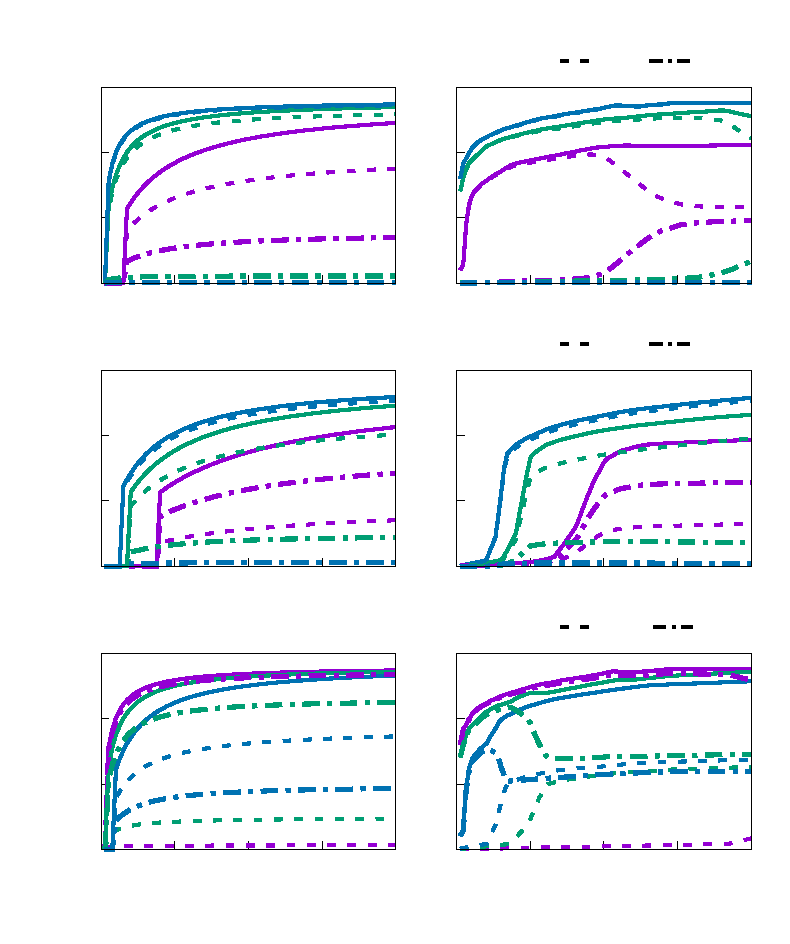
\includegraphics{cu-dhbc-loadings}}%
    \gplfronttext
  \end{picture}%
\endgroup

    \caption{Total (full lines) and partial (dashed lines) loading as function
    of pressure in \Cudhbc for all the gas pairs: from top to bottom \ce{CO2} /
    \ce{O2}; \ce{CH4} / \ce{O2}; and \ce{CH4} / \ce{CO2}. OFAST results are
    presented on the left, and IAST results on the right.}
    \label{fig:cu-dhbc:iast-ofast:loadings}
\end{figure}

In stark contrast with this picture, the selectivities calculated by IAST are
clearly non-physical. All selectivity curves present a maximum in the pressure
range where gate opening occurs, with selectivities that can be several orders
of magnitude too high, with for example 2 000 instead of 20 for
\ce{CO2}/\ce{O2}. Even at higher pressure --- above the gate opening pressure
range --- the behavior is not identical to the OFAST calculations, because the
incorrect behavior at low pressure affects IAST directly in the integration of
the isotherms (equation~\eqref{eq:iast}).

Moreover, the IAST selectivity for \ce{CO2}/\ce{O2} presents a big jump around
\SI{40}{atm} when $y_{\ce{CO2}} = 0.1$. Looking at the partial loading in
figure~\ref{fig:cu-dhbc:iast-ofast:loadings} top right panel, we can attribute
this jump to an equilibrium displacement: \ce{O2} is replacing \ce{CO2} in the
structure. This shows again the fact that IAST behaves as if the structure was
closed for \ce{O2} while at the same time being open for \ce{CO2} at pressures
lower than \SI{40}{atm}. I thus confirm by a quantitative study that IAST is not
adapted for adsorption in flexible nanoporous materials.

\FloatBarrier
\subsubsection{More complex isotherms: the case of \RPMZn}

\begin{figure}[htp]
    \centering
    \raisebox{-0.5\height}{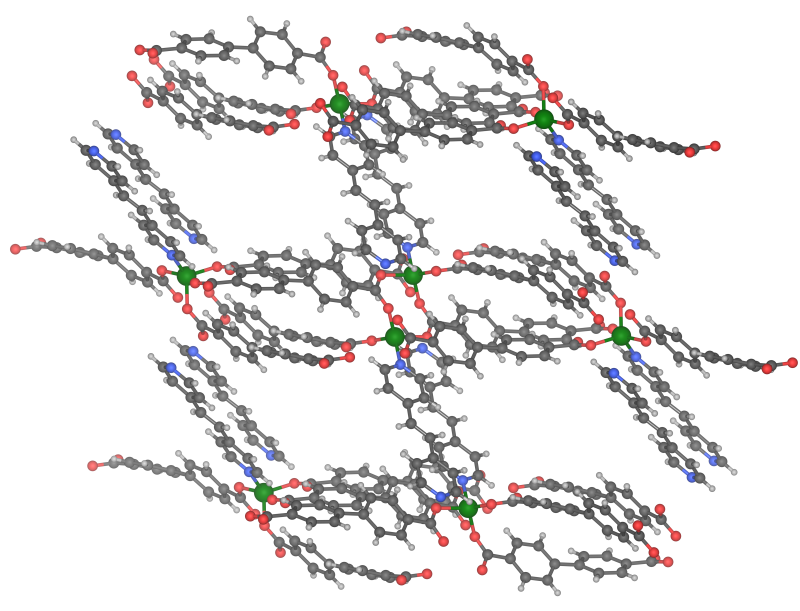
\includegraphics[width=0.35\textwidth]{figures/images/rpm3-zn-structure}}
    \hfill
    \raisebox{-0.5\height}{% GNUPLOT: LaTeX picture with Postscript
\begingroup
  \makeatletter
  \providecommand\color[2][]{%
    \GenericError{(gnuplot) \space\space\space\@spaces}{%
      Package color not loaded in conjunction with
      terminal option `colourtext'%
    }{See the gnuplot documentation for explanation.%
    }{Either use 'blacktext' in gnuplot or load the package
      color.sty in LaTeX.}%
    \renewcommand\color[2][]{}%
  }%
  \providecommand\includegraphics[2][]{%
    \GenericError{(gnuplot) \space\space\space\@spaces}{%
      Package graphicx or graphics not loaded%
    }{See the gnuplot documentation for explanation.%
    }{The gnuplot epslatex terminal needs graphicx.sty or graphics.sty.}%
    \renewcommand\includegraphics[2][]{}%
  }%
  \providecommand\rotatebox[2]{#2}%
  \@ifundefined{ifGPcolor}{%
    \newif\ifGPcolor
    \GPcolortrue
  }{}%
  \@ifundefined{ifGPblacktext}{%
    \newif\ifGPblacktext
    \GPblacktextfalse
  }{}%
  % define a \g@addto@macro without @ in the name:
  \let\gplgaddtomacro\g@addto@macro
  % define empty templates for all commands taking text:
  \gdef\gplbacktext{}%
  \gdef\gplfronttext{}%
  \makeatother
  \ifGPblacktext
    % no textcolor at all
    \def\colorrgb#1{}%
    \def\colorgray#1{}%
  \else
    % gray or color?
    \ifGPcolor
      \def\colorrgb#1{\color[rgb]{#1}}%
      \def\colorgray#1{\color[gray]{#1}}%
      \expandafter\def\csname LTw\endcsname{\color{white}}%
      \expandafter\def\csname LTb\endcsname{\color{black}}%
      \expandafter\def\csname LTa\endcsname{\color{black}}%
      \expandafter\def\csname LT0\endcsname{\color[rgb]{1,0,0}}%
      \expandafter\def\csname LT1\endcsname{\color[rgb]{0,1,0}}%
      \expandafter\def\csname LT2\endcsname{\color[rgb]{0,0,1}}%
      \expandafter\def\csname LT3\endcsname{\color[rgb]{1,0,1}}%
      \expandafter\def\csname LT4\endcsname{\color[rgb]{0,1,1}}%
      \expandafter\def\csname LT5\endcsname{\color[rgb]{1,1,0}}%
      \expandafter\def\csname LT6\endcsname{\color[rgb]{0,0,0}}%
      \expandafter\def\csname LT7\endcsname{\color[rgb]{1,0.3,0}}%
      \expandafter\def\csname LT8\endcsname{\color[rgb]{0.5,0.5,0.5}}%
    \else
      % gray
      \def\colorrgb#1{\color{black}}%
      \def\colorgray#1{\color[gray]{#1}}%
      \expandafter\def\csname LTw\endcsname{\color{white}}%
      \expandafter\def\csname LTb\endcsname{\color{black}}%
      \expandafter\def\csname LTa\endcsname{\color{black}}%
      \expandafter\def\csname LT0\endcsname{\color{black}}%
      \expandafter\def\csname LT1\endcsname{\color{black}}%
      \expandafter\def\csname LT2\endcsname{\color{black}}%
      \expandafter\def\csname LT3\endcsname{\color{black}}%
      \expandafter\def\csname LT4\endcsname{\color{black}}%
      \expandafter\def\csname LT5\endcsname{\color{black}}%
      \expandafter\def\csname LT6\endcsname{\color{black}}%
      \expandafter\def\csname LT7\endcsname{\color{black}}%
      \expandafter\def\csname LT8\endcsname{\color{black}}%
    \fi
  \fi
    \setlength{\unitlength}{0.0500bp}%
    \ifx\gptboxheight\undefined%
      \newlength{\gptboxheight}%
      \newlength{\gptboxwidth}%
      \newsavebox{\gptboxtext}%
    \fi%
    \setlength{\fboxrule}{0.5pt}%
    \setlength{\fboxsep}{1pt}%
\begin{picture}(4520.00,3400.00)%
    \gplgaddtomacro\gplbacktext{%
      \csname LTb\endcsname%%
      \put(543,833){\makebox(0,0)[r]{\strut{}$0$}}%
      \csname LTb\endcsname%%
      \put(543,1309){\makebox(0,0)[r]{\strut{}$2$}}%
      \csname LTb\endcsname%%
      \put(543,1785){\makebox(0,0)[r]{\strut{}$4$}}%
      \csname LTb\endcsname%%
      \put(543,2261){\makebox(0,0)[r]{\strut{}$6$}}%
      \csname LTb\endcsname%%
      \put(543,2737){\makebox(0,0)[r]{\strut{}$8$}}%
      \csname LTb\endcsname%%
      \put(543,3213){\makebox(0,0)[r]{\strut{}$10$}}%
      \csname LTb\endcsname%%
      \put(645,409){\makebox(0,0){\strut{}$0.001$}}%
      \csname LTb\endcsname%%
      \put(1834,409){\makebox(0,0){\strut{}$0.01$}}%
      \csname LTb\endcsname%%
      \put(3024,409){\makebox(0,0){\strut{}$0.1$}}%
      \csname LTb\endcsname%%
      \put(4213,409){\makebox(0,0){\strut{}$1$}}%
    }%
    \gplgaddtomacro\gplfronttext{%
      \csname LTb\endcsname%%
      \put(153,1904){\rotatebox{-270}{\makebox(0,0){\strut{}uptake / (mol/mol)}}}%
      \csname LTb\endcsname%%
      \put(2429,130){\makebox(0,0){\strut{}pressure / bar}}%
      \csname LTb\endcsname%%
      \put(1359,3018){\makebox(0,0)[r]{\strut{}\ce{C2H6}}}%
      \csname LTb\endcsname%%
      \put(1359,2777){\makebox(0,0)[r]{\strut{}\ce{C3H8}}}%
      \csname LTb\endcsname%%
      \put(1359,2536){\makebox(0,0)[r]{\strut{}\ce{C4H10}}}%
    }%
    \gplbacktext
    \put(0,0){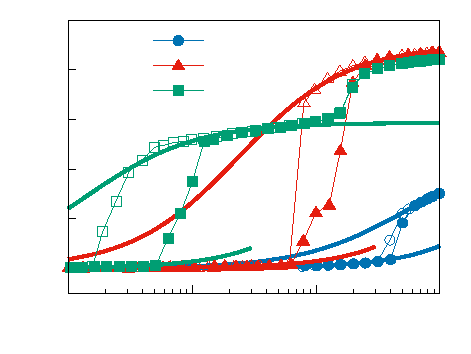
\includegraphics{rpm3-zn}}%
    \gplfronttext
  \end{picture}%
\endgroup
}
    \caption{(left) \RPMZn structure (from reference~\cite{Lan2009-2}).
    (right) Sorption isotherms at \SI{298}{K} for short
    alkanes in \RPMZn. Blue circles are for \ce{C2H6}, red triangles for
    \ce{C3H8}, and green squares for \ce{C4H10}. Filled symbols for adsorption,
    empty symbols for desorption. Thick lines are the open and closed phases fit
    of the isotherms. Experimental data published by
    \citeauthor{Nijem2012}\cite{Nijem2012}}
    \label{fig:rpm3-zn}
\end{figure}

We now turn to a second example of gate opening material, \RPMZn\cite{Lan2009-2},
which presents more complex adsorption--desorption isotherms for short alkanes
(ethane, propane, butane) --- depicted on the right panel of
figure~\ref{fig:rpm3-zn}. While adsorption of \ce{C2H6}, and \ce{C3H8} in this
material displays a typical gate opening behavior, with a well-marked single
transition from a nonporous to a microporous phase, the adsorption of \ce{C4H10}
presents two steps at \SI{0.01}{atm} and \SI{0.2}{atm}. There, the first
transition can be attributed to the structural transition (gate opening), but
the second one is of a different nature. Because there is no hysteresis loop for
the second step, and because it occurs for the larger and more anisotropic guest
molecule, it can be attributed to a fluid reorganization (or fluid packing)
transition inside the pores. Because experimental \emph{in situ}
characterization (such as single X-ray diffraction) would be necessary to
definitely affirm the character of this second step, I chose avoid the issue and
work in a reduced pressure range --- although the OFAST method itself works with
host materials with more than two phases. I thus fitted the \ce{C4H10} isotherm
using a Langmuir isotherm for pressures below \SI{0.2}{atm}.  The OFAST
selectivity after this pressure will thus not be quantitatively accurate, but
will be sufficient for the needed physical insight. I also performed tests by
computing the selectivity under the assumption that the second jump is due to
fluid reorganization by using Langmuir-Freundlich isotherms instead of single
site Langmuir isotherm in the open phase, and the selectivity only differs at
pressures higher than \SI{0.2}{atm}.

\begin{table}[htp]
    \renewcommand{\arraystretch}{1.3}
    \newcolumntype{C}{>{\centering\arraybackslash}X}
    \begin{tabularx}{\textwidth}{c C c C c C}
        \textbf{Gas} & $K_H$ / (mol/bar) & $N_L$ / mol & $K_L$ / bar & $P_\text{trans}$ / bar & $\Delta F$ / (kJ/mol)  \\ \hline
        \ce{C2H6}    & 0.905             & 4.82        & 1.74        &            /           &          /             \\
        \ce{C3H8}    & 2.88              & 9.00        & 42.0        &           0.07         &        -30.1           \\
        \ce{C4H10}   & 27.3              & 5.87        & 699         &           0.01         &        -29.8           \\
    \end{tabularx}
    \caption{Fitted coefficients for the sorption isotherms and free energy
    difference between open and closed structures in \RPMZn. See
    equations~\eqref{eq:henry-isotherm} and \eqref{eq:langmuir-isotherm} for the
    definitions of $K_H$, $N_L$ and $K_L$.}
    \label{table:rpm3-zn:fit}
\end{table}

From the \ce{C3H8} and \ce{C4H10} isotherms, I computed the free energy
difference between the nonporous and microporous phases, which I find to be
$\Delta F = -30.0 \pm \SI{0.1}{kJ/mol}$. The details are in
table~\ref{table:rpm3-zn:fit}. I did not use the \ce{C2H6} isotherms for this
purpose, as it has only limited data at high loading (at pressure above 1 bar),
which increases somewhat the uncertainty of the fit. I was still able to fit the
\ce{C2H6} isotherm with a Langmuir model and use it to compute co-adsorption
data, as the free energy difference of the two host phases do not depend on the
gas.

\begin{figure}[htp]
    \centering
    % GNUPLOT: LaTeX picture with Postscript
\begingroup
  \makeatletter
  \providecommand\color[2][]{%
    \GenericError{(gnuplot) \space\space\space\@spaces}{%
      Package color not loaded in conjunction with
      terminal option `colourtext'%
    }{See the gnuplot documentation for explanation.%
    }{Either use 'blacktext' in gnuplot or load the package
      color.sty in LaTeX.}%
    \renewcommand\color[2][]{}%
  }%
  \providecommand\includegraphics[2][]{%
    \GenericError{(gnuplot) \space\space\space\@spaces}{%
      Package graphicx or graphics not loaded%
    }{See the gnuplot documentation for explanation.%
    }{The gnuplot epslatex terminal needs graphicx.sty or graphics.sty.}%
    \renewcommand\includegraphics[2][]{}%
  }%
  \providecommand\rotatebox[2]{#2}%
  \@ifundefined{ifGPcolor}{%
    \newif\ifGPcolor
    \GPcolortrue
  }{}%
  \@ifundefined{ifGPblacktext}{%
    \newif\ifGPblacktext
    \GPblacktextfalse
  }{}%
  % define a \g@addto@macro without @ in the name:
  \let\gplgaddtomacro\g@addto@macro
  % define empty templates for all commands taking text:
  \gdef\gplbacktext{}%
  \gdef\gplfronttext{}%
  \makeatother
  \ifGPblacktext
    % no textcolor at all
    \def\colorrgb#1{}%
    \def\colorgray#1{}%
  \else
    % gray or color?
    \ifGPcolor
      \def\colorrgb#1{\color[rgb]{#1}}%
      \def\colorgray#1{\color[gray]{#1}}%
      \expandafter\def\csname LTw\endcsname{\color{white}}%
      \expandafter\def\csname LTb\endcsname{\color{black}}%
      \expandafter\def\csname LTa\endcsname{\color{black}}%
      \expandafter\def\csname LT0\endcsname{\color[rgb]{1,0,0}}%
      \expandafter\def\csname LT1\endcsname{\color[rgb]{0,1,0}}%
      \expandafter\def\csname LT2\endcsname{\color[rgb]{0,0,1}}%
      \expandafter\def\csname LT3\endcsname{\color[rgb]{1,0,1}}%
      \expandafter\def\csname LT4\endcsname{\color[rgb]{0,1,1}}%
      \expandafter\def\csname LT5\endcsname{\color[rgb]{1,1,0}}%
      \expandafter\def\csname LT6\endcsname{\color[rgb]{0,0,0}}%
      \expandafter\def\csname LT7\endcsname{\color[rgb]{1,0.3,0}}%
      \expandafter\def\csname LT8\endcsname{\color[rgb]{0.5,0.5,0.5}}%
    \else
      % gray
      \def\colorrgb#1{\color{black}}%
      \def\colorgray#1{\color[gray]{#1}}%
      \expandafter\def\csname LTw\endcsname{\color{white}}%
      \expandafter\def\csname LTb\endcsname{\color{black}}%
      \expandafter\def\csname LTa\endcsname{\color{black}}%
      \expandafter\def\csname LT0\endcsname{\color{black}}%
      \expandafter\def\csname LT1\endcsname{\color{black}}%
      \expandafter\def\csname LT2\endcsname{\color{black}}%
      \expandafter\def\csname LT3\endcsname{\color{black}}%
      \expandafter\def\csname LT4\endcsname{\color{black}}%
      \expandafter\def\csname LT5\endcsname{\color{black}}%
      \expandafter\def\csname LT6\endcsname{\color{black}}%
      \expandafter\def\csname LT7\endcsname{\color{black}}%
      \expandafter\def\csname LT8\endcsname{\color{black}}%
    \fi
  \fi
    \setlength{\unitlength}{0.0500bp}%
    \ifx\gptboxheight\undefined%
      \newlength{\gptboxheight}%
      \newlength{\gptboxwidth}%
      \newsavebox{\gptboxtext}%
    \fi%
    \setlength{\fboxrule}{0.5pt}%
    \setlength{\fboxsep}{1pt}%
\begin{picture}(7360.00,2820.00)%
    \gplgaddtomacro\gplbacktext{%
      \csname LTb\endcsname%%
      \put(498,396){\makebox(0,0)[r]{\strut{}\footnotesize$10^{0}$}}%
      \csname LTb\endcsname%%
      \put(498,1080){\makebox(0,0)[r]{\strut{}\footnotesize$10^{1}$}}%
      \csname LTb\endcsname%%
      \put(498,1763){\makebox(0,0)[r]{\strut{}\footnotesize$10^{2}$}}%
      \csname LTb\endcsname%%
      \put(498,2447){\makebox(0,0)[r]{\strut{}\footnotesize$10^{3}$}}%
      \csname LTb\endcsname%%
      \put(566,248){\makebox(0,0){\strut{}\footnotesize$10^{-3}$}}%
      \csname LTb\endcsname%%
      \put(1127,248){\makebox(0,0){\strut{}\footnotesize$10^{-2}$}}%
      \csname LTb\endcsname%%
      \put(1688,248){\makebox(0,0){\strut{}\footnotesize$10^{-1}$}}%
      \csname LTb\endcsname%%
      \put(2249,248){\makebox(0,0){\strut{}\footnotesize$10^{0}$}}%
    }%
    \gplgaddtomacro\gplfronttext{%
      \csname LTb\endcsname%%
      \put(102,1421){\rotatebox{-270}{\makebox(0,0){\strut{}\small selectivity}}}%
      \csname LTb\endcsname%%
      \put(1407,86){\makebox(0,0){\strut{}\small pressure / bar}}%
      \csname LTb\endcsname%%
      \put(1407,2633){\makebox(0,0){\strut{}\ce{C3H8} / \ce{C2H6}}}%
      \csname LTb\endcsname%%
      \put(1382,2305){\makebox(0,0)[r]{\strut{}\footnotesize$y_{\smallce{C3}} = 0.1$}}%
      \csname LTb\endcsname%%
      \put(1382,2119){\makebox(0,0)[r]{\strut{}\footnotesize$y_{\smallce{C3}} = 0.5$}}%
      \csname LTb\endcsname%%
      \put(1382,1933){\makebox(0,0)[r]{\strut{}\footnotesize$y_{\smallce{C3}} = 0.9$}}%
    }%
    \gplgaddtomacro\gplbacktext{%
      \csname LTb\endcsname%%
      \put(2827,396){\makebox(0,0)[r]{\strut{}\footnotesize$10^{0}$}}%
      \csname LTb\endcsname%%
      \put(2827,1422){\makebox(0,0)[r]{\strut{}\footnotesize$10^{1}$}}%
      \csname LTb\endcsname%%
      \put(2827,2447){\makebox(0,0)[r]{\strut{}\footnotesize$10^{2}$}}%
      \csname LTb\endcsname%%
      \put(2895,248){\makebox(0,0){\strut{}\footnotesize$10^{-3}$}}%
      \csname LTb\endcsname%%
      \put(3497,248){\makebox(0,0){\strut{}\footnotesize$10^{-2}$}}%
      \csname LTb\endcsname%%
      \put(4100,248){\makebox(0,0){\strut{}\footnotesize$10^{-1}$}}%
      \csname LTb\endcsname%%
      \put(4702,248){\makebox(0,0){\strut{}\footnotesize$10^{0}$}}%
    }%
    \gplgaddtomacro\gplfronttext{%
      \csname LTb\endcsname%%
      \put(3798,86){\makebox(0,0){\strut{}\small pressure / bar}}%
      \csname LTb\endcsname%%
      \put(3798,2633){\makebox(0,0){\strut{}\ce{C4H10} / \ce{C3H8}}}%
      \csname LTb\endcsname%%
      \put(4381,2305){\makebox(0,0)[r]{\strut{}\footnotesize$y_{\smallce{C4}} = 0.1$}}%
      \csname LTb\endcsname%%
      \put(4381,2119){\makebox(0,0)[r]{\strut{}\footnotesize$y_{\smallce{C4}} = 0.5$}}%
      \csname LTb\endcsname%%
      \put(4381,1933){\makebox(0,0)[r]{\strut{}\footnotesize$y_{\smallce{C4}} = 0.9$}}%
    }%
    \gplgaddtomacro\gplbacktext{%
      \csname LTb\endcsname%%
      \put(5280,396){\makebox(0,0)[r]{\strut{}\footnotesize$10^{1}$}}%
      \csname LTb\endcsname%%
      \put(5280,1080){\makebox(0,0)[r]{\strut{}\footnotesize$10^{2}$}}%
      \csname LTb\endcsname%%
      \put(5280,1763){\makebox(0,0)[r]{\strut{}\footnotesize$10^{3}$}}%
      \csname LTb\endcsname%%
      \put(5280,2447){\makebox(0,0)[r]{\strut{}\footnotesize$10^{4}$}}%
      \csname LTb\endcsname%%
      \put(5348,248){\makebox(0,0){\strut{}\footnotesize$10^{-3}$}}%
      \csname LTb\endcsname%%
      \put(5950,248){\makebox(0,0){\strut{}\footnotesize$10^{-2}$}}%
      \csname LTb\endcsname%%
      \put(6553,248){\makebox(0,0){\strut{}\footnotesize$10^{-1}$}}%
      \csname LTb\endcsname%%
      \put(7155,248){\makebox(0,0){\strut{}\footnotesize$10^{0}$}}%
    }%
    \gplgaddtomacro\gplfronttext{%
      \csname LTb\endcsname%%
      \put(6251,86){\makebox(0,0){\strut{}\small pressure / bar}}%
      \csname LTb\endcsname%%
      \put(6251,2633){\makebox(0,0){\strut{}\ce{C4H10} / \ce{C2H6}}}%
      \csname LTb\endcsname%%
      \put(6499,2305){\makebox(0,0)[r]{\strut{}\footnotesize$y_{\smallce{C4}} = 0.1$}}%
      \csname LTb\endcsname%%
      \put(6499,2119){\makebox(0,0)[r]{\strut{}\footnotesize$y_{\smallce{C4}} = 0.5$}}%
      \csname LTb\endcsname%%
      \put(6499,1933){\makebox(0,0)[r]{\strut{}\footnotesize$y_{\smallce{C4}} = 0.9$}}%
    }%
    \gplbacktext
    \put(0,0){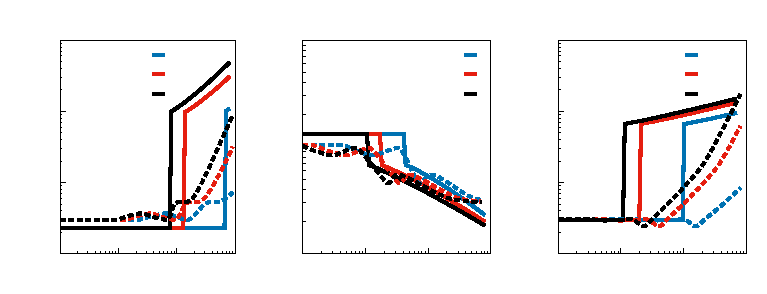
\includegraphics{rpm3-zn-selectivities}}%
    \gplfronttext
  \end{picture}%
\endgroup

    \caption{IAST (dashed lines) vs OFAST (plain lines) adsorption selectivity
    for \ce{C3H8}/\ce{C2H6} (left) and \ce{C4H10}/\ce{C3H8} (right) mixtures
    in \RPMZn at different compositions.}
    \label{fig:rpm3-zn:iast-ofast:selectivity}
\end{figure}

Figure~\ref{fig:rpm3-zn:iast-ofast:selectivity} displays the selectivity curves
obtained with IAST and OFAST for various gas mixtures and compositions in
\RPMZn; and figure~\ref{fig:rpm3-zn:iast-ofast:loadings} shows the partial and
total loading predicted by both methods. Again, the OFAST selectivity curve
follows the expected behavior: it is constant at low loading, where
single-component isotherms follow the Henry model. In this low-pressure region,
adsorption is negligible and the selectivity cannot be exploited in
adsorption-based processes. However, we can see that because IAST is using
numerical integration, it is much more sensitive to details in the
single-component isotherms than the OFAST method, which is based on fits.

\begin{figure}[htp]
    \centering
    % GNUPLOT: LaTeX picture with Postscript
\begingroup
  \makeatletter
  \providecommand\color[2][]{%
    \GenericError{(gnuplot) \space\space\space\@spaces}{%
      Package color not loaded in conjunction with
      terminal option `colourtext'%
    }{See the gnuplot documentation for explanation.%
    }{Either use 'blacktext' in gnuplot or load the package
      color.sty in LaTeX.}%
    \renewcommand\color[2][]{}%
  }%
  \providecommand\includegraphics[2][]{%
    \GenericError{(gnuplot) \space\space\space\@spaces}{%
      Package graphicx or graphics not loaded%
    }{See the gnuplot documentation for explanation.%
    }{The gnuplot epslatex terminal needs graphicx.sty or graphics.sty.}%
    \renewcommand\includegraphics[2][]{}%
  }%
  \providecommand\rotatebox[2]{#2}%
  \@ifundefined{ifGPcolor}{%
    \newif\ifGPcolor
    \GPcolortrue
  }{}%
  \@ifundefined{ifGPblacktext}{%
    \newif\ifGPblacktext
    \GPblacktextfalse
  }{}%
  % define a \g@addto@macro without @ in the name:
  \let\gplgaddtomacro\g@addto@macro
  % define empty templates for all commands taking text:
  \gdef\gplbacktext{}%
  \gdef\gplfronttext{}%
  \makeatother
  \ifGPblacktext
    % no textcolor at all
    \def\colorrgb#1{}%
    \def\colorgray#1{}%
  \else
    % gray or color?
    \ifGPcolor
      \def\colorrgb#1{\color[rgb]{#1}}%
      \def\colorgray#1{\color[gray]{#1}}%
      \expandafter\def\csname LTw\endcsname{\color{white}}%
      \expandafter\def\csname LTb\endcsname{\color{black}}%
      \expandafter\def\csname LTa\endcsname{\color{black}}%
      \expandafter\def\csname LT0\endcsname{\color[rgb]{1,0,0}}%
      \expandafter\def\csname LT1\endcsname{\color[rgb]{0,1,0}}%
      \expandafter\def\csname LT2\endcsname{\color[rgb]{0,0,1}}%
      \expandafter\def\csname LT3\endcsname{\color[rgb]{1,0,1}}%
      \expandafter\def\csname LT4\endcsname{\color[rgb]{0,1,1}}%
      \expandafter\def\csname LT5\endcsname{\color[rgb]{1,1,0}}%
      \expandafter\def\csname LT6\endcsname{\color[rgb]{0,0,0}}%
      \expandafter\def\csname LT7\endcsname{\color[rgb]{1,0.3,0}}%
      \expandafter\def\csname LT8\endcsname{\color[rgb]{0.5,0.5,0.5}}%
    \else
      % gray
      \def\colorrgb#1{\color{black}}%
      \def\colorgray#1{\color[gray]{#1}}%
      \expandafter\def\csname LTw\endcsname{\color{white}}%
      \expandafter\def\csname LTb\endcsname{\color{black}}%
      \expandafter\def\csname LTa\endcsname{\color{black}}%
      \expandafter\def\csname LT0\endcsname{\color{black}}%
      \expandafter\def\csname LT1\endcsname{\color{black}}%
      \expandafter\def\csname LT2\endcsname{\color{black}}%
      \expandafter\def\csname LT3\endcsname{\color{black}}%
      \expandafter\def\csname LT4\endcsname{\color{black}}%
      \expandafter\def\csname LT5\endcsname{\color{black}}%
      \expandafter\def\csname LT6\endcsname{\color{black}}%
      \expandafter\def\csname LT7\endcsname{\color{black}}%
      \expandafter\def\csname LT8\endcsname{\color{black}}%
    \fi
  \fi
    \setlength{\unitlength}{0.0500bp}%
    \ifx\gptboxheight\undefined%
      \newlength{\gptboxheight}%
      \newlength{\gptboxwidth}%
      \newsavebox{\gptboxtext}%
    \fi%
    \setlength{\fboxrule}{0.5pt}%
    \setlength{\fboxsep}{1pt}%
\begin{picture}(7580.00,8500.00)%
    \gplgaddtomacro\gplbacktext{%
      \csname LTb\endcsname%%
      \put(860,5990){\makebox(0,0)[r]{\strut{}\small 0}}%
      \csname LTb\endcsname%%
      \put(860,6407){\makebox(0,0)[r]{\strut{}\small 2}}%
      \csname LTb\endcsname%%
      \put(860,6824){\makebox(0,0)[r]{\strut{}\small 4}}%
      \csname LTb\endcsname%%
      \put(860,7240){\makebox(0,0)[r]{\strut{}\small 6}}%
      \csname LTb\endcsname%%
      \put(860,7657){\makebox(0,0)[r]{\strut{}\small 8}}%
      \csname LTb\endcsname%%
      \put(860,8074){\makebox(0,0)[r]{\strut{}\small 10}}%
      \csname LTb\endcsname%%
      \put(962,5804){\makebox(0,0){\strut{}\small $10^{-3}$}}%
      \csname LTb\endcsname%%
      \put(1904,5804){\makebox(0,0){\strut{}\small $10^{-2}$}}%
      \csname LTb\endcsname%%
      \put(2847,5804){\makebox(0,0){\strut{}\small $10^{-1}$}}%
      \csname LTb\endcsname%%
      \put(3789,5804){\makebox(0,0){\strut{}\small $10^{0}$}}%
      \csname LTb\endcsname%%
      \put(1971,8329){\makebox(0,0)[l]{\strut{}OFAST}}%
      \csname LTb\endcsname%%
      \put(5457,8329){\makebox(0,0)[l]{\strut{}IAST}}%
      \csname LTb\endcsname%%
      \put(152,6204){\rotatebox{-270}{\makebox(0,0)[l]{\strut{}\ce{C4H10} / \ce{C3H8}}}}%
      \csname LTb\endcsname%%
      \put(152,3740){\rotatebox{-270}{\makebox(0,0)[l]{\strut{}\ce{C3H8} / \ce{C2H6}}}}%
      \csname LTb\endcsname%%
      \put(152,1190){\rotatebox{-270}{\makebox(0,0)[l]{\strut{}\ce{C4H10} / \ce{C2H6}}}}%
    }%
    \gplgaddtomacro\gplfronttext{%
      \csname LTb\endcsname%%
      \put(470,7032){\rotatebox{-270}{\makebox(0,0){\strut{}uptake (mol/mol)}}}%
      \colorrgb{0.58,0.00,0.83}%%
      \put(2030,7773){\makebox(0,0)[r]{\strut{}\footnotesize $y_\smallce{C4H10} = 0.1$}}%
      \colorrgb{0.00,0.62,0.45}%%
      \put(2030,7587){\makebox(0,0)[r]{\strut{}\footnotesize $y_\smallce{C4H10} = 0.5$}}%
      \colorrgb{0.00,0.45,0.70}%%
      \put(2030,7401){\makebox(0,0)[r]{\strut{}\footnotesize $y_\smallce{C4H10} = 0.9$}}%
    }%
    \gplgaddtomacro\gplbacktext{%
      \csname LTb\endcsname%%
      \put(4271,5990){\makebox(0,0)[r]{\strut{}\small 0}}%
      \csname LTb\endcsname%%
      \put(4271,6407){\makebox(0,0)[r]{\strut{}\small 2}}%
      \csname LTb\endcsname%%
      \put(4271,6824){\makebox(0,0)[r]{\strut{}\small 4}}%
      \csname LTb\endcsname%%
      \put(4271,7240){\makebox(0,0)[r]{\strut{}\small 6}}%
      \csname LTb\endcsname%%
      \put(4271,7657){\makebox(0,0)[r]{\strut{}\small 8}}%
      \csname LTb\endcsname%%
      \put(4271,8074){\makebox(0,0)[r]{\strut{}\small 10}}%
      \csname LTb\endcsname%%
      \put(4373,5804){\makebox(0,0){\strut{}\small $10^{-3}$}}%
      \csname LTb\endcsname%%
      \put(5315,5804){\makebox(0,0){\strut{}\small $10^{-2}$}}%
      \csname LTb\endcsname%%
      \put(6258,5804){\makebox(0,0){\strut{}\small $10^{-1}$}}%
      \csname LTb\endcsname%%
      \put(7200,5804){\makebox(0,0){\strut{}\small $10^{0}$}}%
      \csname LTb\endcsname%%
      \put(1971,8329){\makebox(0,0)[l]{\strut{}OFAST}}%
      \csname LTb\endcsname%%
      \put(5457,8329){\makebox(0,0)[l]{\strut{}IAST}}%
      \csname LTb\endcsname%%
      \put(152,6204){\rotatebox{-270}{\makebox(0,0)[l]{\strut{}\ce{C4H10} / \ce{C3H8}}}}%
      \csname LTb\endcsname%%
      \put(152,3740){\rotatebox{-270}{\makebox(0,0)[l]{\strut{}\ce{C3H8} / \ce{C2H6}}}}%
      \csname LTb\endcsname%%
      \put(152,1190){\rotatebox{-270}{\makebox(0,0)[l]{\strut{}\ce{C4H10} / \ce{C2H6}}}}%
    }%
    \gplgaddtomacro\gplfronttext{%
      \colorrgb{0.00,0.00,0.00}%%
      \put(5061,7773){\makebox(0,0)[r]{\strut{}$n_\smallce{C4H10}$}}%
      \colorrgb{0.00,0.00,0.00}%%
      \put(5061,7587){\makebox(0,0)[r]{\strut{}$n_\smallce{C3H8}$}}%
    }%
    \gplgaddtomacro\gplbacktext{%
      \csname LTb\endcsname%%
      \put(860,3440){\makebox(0,0)[r]{\strut{}\small 0}}%
      \csname LTb\endcsname%%
      \put(860,3857){\makebox(0,0)[r]{\strut{}\small 2}}%
      \csname LTb\endcsname%%
      \put(860,4274){\makebox(0,0)[r]{\strut{}\small 4}}%
      \csname LTb\endcsname%%
      \put(860,4690){\makebox(0,0)[r]{\strut{}\small 6}}%
      \csname LTb\endcsname%%
      \put(860,5107){\makebox(0,0)[r]{\strut{}\small 8}}%
      \csname LTb\endcsname%%
      \put(860,5524){\makebox(0,0)[r]{\strut{}\small 10}}%
      \csname LTb\endcsname%%
      \put(962,3254){\makebox(0,0){\strut{}\small $10^{-3}$}}%
      \csname LTb\endcsname%%
      \put(1904,3254){\makebox(0,0){\strut{}\small $10^{-2}$}}%
      \csname LTb\endcsname%%
      \put(2847,3254){\makebox(0,0){\strut{}\small $10^{-1}$}}%
      \csname LTb\endcsname%%
      \put(3789,3254){\makebox(0,0){\strut{}\small $10^{0}$}}%
      \csname LTb\endcsname%%
      \put(1971,8329){\makebox(0,0)[l]{\strut{}OFAST}}%
      \csname LTb\endcsname%%
      \put(5457,8329){\makebox(0,0)[l]{\strut{}IAST}}%
      \csname LTb\endcsname%%
      \put(152,6204){\rotatebox{-270}{\makebox(0,0)[l]{\strut{}\ce{C4H10} / \ce{C3H8}}}}%
      \csname LTb\endcsname%%
      \put(152,3740){\rotatebox{-270}{\makebox(0,0)[l]{\strut{}\ce{C3H8} / \ce{C2H6}}}}%
      \csname LTb\endcsname%%
      \put(152,1190){\rotatebox{-270}{\makebox(0,0)[l]{\strut{}\ce{C4H10} / \ce{C2H6}}}}%
    }%
    \gplgaddtomacro\gplfronttext{%
      \csname LTb\endcsname%%
      \put(470,4482){\rotatebox{-270}{\makebox(0,0){\strut{}uptake (mol/mol)}}}%
      \colorrgb{0.58,0.00,0.83}%%
      \put(2030,5223){\makebox(0,0)[r]{\strut{}\footnotesize $y_\smallce{C3H8} = 0.1$}}%
      \colorrgb{0.00,0.62,0.45}%%
      \put(2030,5037){\makebox(0,0)[r]{\strut{}\footnotesize $y_\smallce{C3H8} = 0.5$}}%
      \colorrgb{0.00,0.45,0.70}%%
      \put(2030,4851){\makebox(0,0)[r]{\strut{}\footnotesize $y_\smallce{C3H8} = 0.9$}}%
    }%
    \gplgaddtomacro\gplbacktext{%
      \csname LTb\endcsname%%
      \put(4271,3440){\makebox(0,0)[r]{\strut{}\small 0}}%
      \csname LTb\endcsname%%
      \put(4271,3857){\makebox(0,0)[r]{\strut{}\small 2}}%
      \csname LTb\endcsname%%
      \put(4271,4274){\makebox(0,0)[r]{\strut{}\small 4}}%
      \csname LTb\endcsname%%
      \put(4271,4690){\makebox(0,0)[r]{\strut{}\small 6}}%
      \csname LTb\endcsname%%
      \put(4271,5107){\makebox(0,0)[r]{\strut{}\small 8}}%
      \csname LTb\endcsname%%
      \put(4271,5524){\makebox(0,0)[r]{\strut{}\small 10}}%
      \csname LTb\endcsname%%
      \put(4373,3254){\makebox(0,0){\strut{}\small $10^{-3}$}}%
      \csname LTb\endcsname%%
      \put(5315,3254){\makebox(0,0){\strut{}\small $10^{-2}$}}%
      \csname LTb\endcsname%%
      \put(6258,3254){\makebox(0,0){\strut{}\small $10^{-1}$}}%
      \csname LTb\endcsname%%
      \put(7200,3254){\makebox(0,0){\strut{}\small $10^{0}$}}%
      \csname LTb\endcsname%%
      \put(1971,8329){\makebox(0,0)[l]{\strut{}OFAST}}%
      \csname LTb\endcsname%%
      \put(5457,8329){\makebox(0,0)[l]{\strut{}IAST}}%
      \csname LTb\endcsname%%
      \put(152,6204){\rotatebox{-270}{\makebox(0,0)[l]{\strut{}\ce{C4H10} / \ce{C3H8}}}}%
      \csname LTb\endcsname%%
      \put(152,3740){\rotatebox{-270}{\makebox(0,0)[l]{\strut{}\ce{C3H8} / \ce{C2H6}}}}%
      \csname LTb\endcsname%%
      \put(152,1190){\rotatebox{-270}{\makebox(0,0)[l]{\strut{}\ce{C4H10} / \ce{C2H6}}}}%
    }%
    \gplgaddtomacro\gplfronttext{%
      \colorrgb{0.00,0.00,0.00}%%
      \put(5061,5223){\makebox(0,0)[r]{\strut{}$n_\smallce{C3H8}$}}%
      \colorrgb{0.00,0.00,0.00}%%
      \put(5061,5037){\makebox(0,0)[r]{\strut{}$n_\smallce{C2H6}$}}%
    }%
    \gplgaddtomacro\gplbacktext{%
      \csname LTb\endcsname%%
      \put(860,890){\makebox(0,0)[r]{\strut{}\small 0}}%
      \csname LTb\endcsname%%
      \put(860,1307){\makebox(0,0)[r]{\strut{}\small 2}}%
      \csname LTb\endcsname%%
      \put(860,1724){\makebox(0,0)[r]{\strut{}\small 4}}%
      \csname LTb\endcsname%%
      \put(860,2141){\makebox(0,0)[r]{\strut{}\small 6}}%
      \csname LTb\endcsname%%
      \put(860,2558){\makebox(0,0)[r]{\strut{}\small 8}}%
      \csname LTb\endcsname%%
      \put(860,2975){\makebox(0,0)[r]{\strut{}\small 10}}%
      \csname LTb\endcsname%%
      \put(962,704){\makebox(0,0){\strut{}\small $10^{-3}$}}%
      \csname LTb\endcsname%%
      \put(1904,704){\makebox(0,0){\strut{}\small $10^{-2}$}}%
      \csname LTb\endcsname%%
      \put(2847,704){\makebox(0,0){\strut{}\small $10^{-1}$}}%
      \csname LTb\endcsname%%
      \put(3789,704){\makebox(0,0){\strut{}\small $10^{0}$}}%
      \csname LTb\endcsname%%
      \put(1971,8329){\makebox(0,0)[l]{\strut{}OFAST}}%
      \csname LTb\endcsname%%
      \put(5457,8329){\makebox(0,0)[l]{\strut{}IAST}}%
      \csname LTb\endcsname%%
      \put(152,6204){\rotatebox{-270}{\makebox(0,0)[l]{\strut{}\ce{C4H10} / \ce{C3H8}}}}%
      \csname LTb\endcsname%%
      \put(152,3740){\rotatebox{-270}{\makebox(0,0)[l]{\strut{}\ce{C3H8} / \ce{C2H6}}}}%
      \csname LTb\endcsname%%
      \put(152,1190){\rotatebox{-270}{\makebox(0,0)[l]{\strut{}\ce{C4H10} / \ce{C2H6}}}}%
    }%
    \gplgaddtomacro\gplfronttext{%
      \csname LTb\endcsname%%
      \put(470,1932){\rotatebox{-270}{\makebox(0,0){\strut{}uptake (mol/mol)}}}%
      \csname LTb\endcsname%%
      \put(2477,425){\makebox(0,0){\strut{}pressure / atm}}%
      \colorrgb{0.58,0.00,0.83}%%
      \put(2030,2674){\makebox(0,0)[r]{\strut{}\footnotesize $y_\smallce{C4H10} = 0.1$}}%
      \colorrgb{0.00,0.62,0.45}%%
      \put(2030,2488){\makebox(0,0)[r]{\strut{}\footnotesize $y_\smallce{C4H10} = 0.5$}}%
      \colorrgb{0.00,0.45,0.70}%%
      \put(2030,2302){\makebox(0,0)[r]{\strut{}\footnotesize $y_\smallce{C4H10} = 0.9$}}%
    }%
    \gplgaddtomacro\gplbacktext{%
      \csname LTb\endcsname%%
      \put(4271,890){\makebox(0,0)[r]{\strut{}\small 0}}%
      \csname LTb\endcsname%%
      \put(4271,1307){\makebox(0,0)[r]{\strut{}\small 2}}%
      \csname LTb\endcsname%%
      \put(4271,1724){\makebox(0,0)[r]{\strut{}\small 4}}%
      \csname LTb\endcsname%%
      \put(4271,2141){\makebox(0,0)[r]{\strut{}\small 6}}%
      \csname LTb\endcsname%%
      \put(4271,2558){\makebox(0,0)[r]{\strut{}\small 8}}%
      \csname LTb\endcsname%%
      \put(4271,2975){\makebox(0,0)[r]{\strut{}\small 10}}%
      \csname LTb\endcsname%%
      \put(4373,704){\makebox(0,0){\strut{}\small $10^{-3}$}}%
      \csname LTb\endcsname%%
      \put(5315,704){\makebox(0,0){\strut{}\small $10^{-2}$}}%
      \csname LTb\endcsname%%
      \put(6258,704){\makebox(0,0){\strut{}\small $10^{-1}$}}%
      \csname LTb\endcsname%%
      \put(7200,704){\makebox(0,0){\strut{}\small $10^{0}$}}%
      \csname LTb\endcsname%%
      \put(1971,8329){\makebox(0,0)[l]{\strut{}OFAST}}%
      \csname LTb\endcsname%%
      \put(5457,8329){\makebox(0,0)[l]{\strut{}IAST}}%
      \csname LTb\endcsname%%
      \put(152,6204){\rotatebox{-270}{\makebox(0,0)[l]{\strut{}\ce{C4H10} / \ce{C3H8}}}}%
      \csname LTb\endcsname%%
      \put(152,3740){\rotatebox{-270}{\makebox(0,0)[l]{\strut{}\ce{C3H8} / \ce{C2H6}}}}%
      \csname LTb\endcsname%%
      \put(152,1190){\rotatebox{-270}{\makebox(0,0)[l]{\strut{}\ce{C4H10} / \ce{C2H6}}}}%
    }%
    \gplgaddtomacro\gplfronttext{%
      \csname LTb\endcsname%%
      \put(5888,425){\makebox(0,0){\strut{}pressure / atm}}%
      \colorrgb{0.00,0.00,0.00}%%
      \put(5061,2674){\makebox(0,0)[r]{\strut{}$n_\smallce{C4H10}$}}%
      \colorrgb{0.00,0.00,0.00}%%
      \put(5061,2488){\makebox(0,0)[r]{\strut{}$n_\smallce{C2H6}$}}%
    }%
    \gplbacktext
    \put(0,0){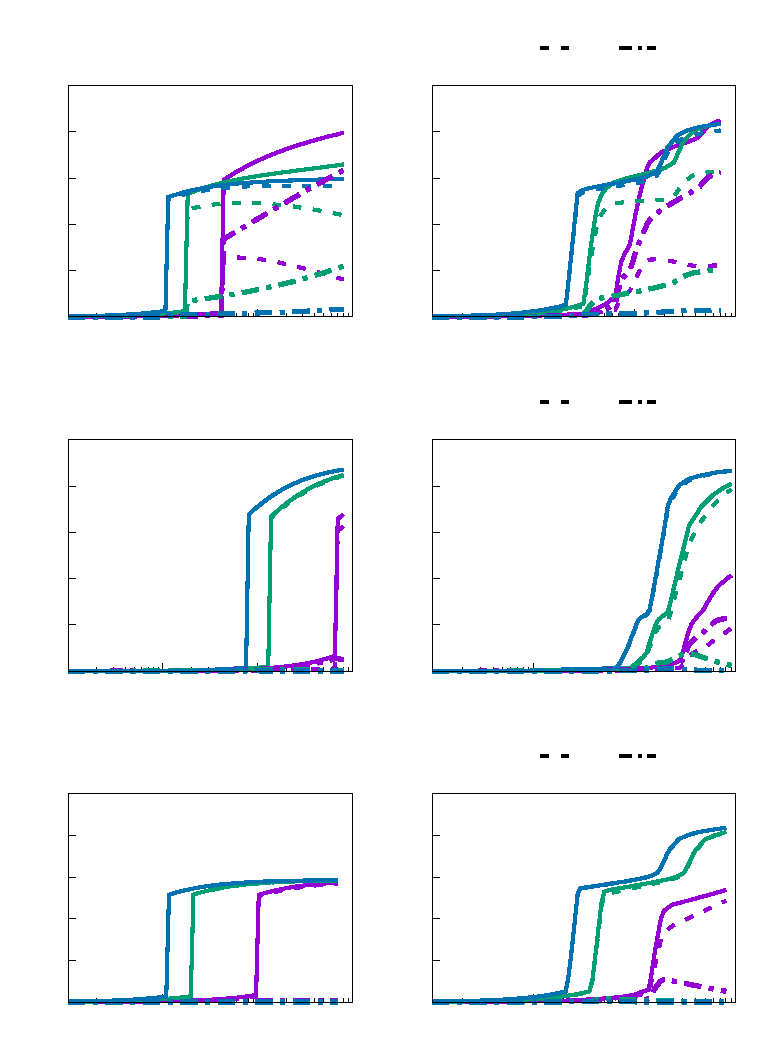
\includegraphics{rpm3-zn-loadings}}%
    \gplfronttext
  \end{picture}%
\endgroup

    \caption{Total (full lines) and partial (dashed lines) loading as function
    of pressure in \RPMZn for all the gas pairs: from top to bottom \ce{C4H10} /
    \ce{C3H8}; \ce{C3H8} / \ce{C2H6}; and \ce{C4H10} / \ce{C2H6}. OFAST results
    are presented on the left, and IAST results on the right.}
    \label{fig:rpm3-zn:iast-ofast:loadings}
\end{figure}

OFAST correctly describes the occurrence of gate opening, at a pressure which
depends on mixture composition but is in the range of the pure component gating
pressures. After gate opening, the selectivity jumps to its value in the open
pore framework. \ce{C3H8}/\ce{C2H6} mixtures have a behavior similar to that
observed in \Cudhbc, with a slowly growing (in logarithmic scale) selectivity at
high loading. On the other hand, OFAST selectivity for \ce{C4H10}/\ce{C3H8}
mixture displays a different behavior. The selectivity is lower after the
transition than before, and further decreases as the pressure and loading
increases. This is due to the fact that the single-component isotherms  in the
open pore structure cross, with \ce{C3H8} adsorbing more than \ce{C4H10} for
pressure bigger than \SI{0.03}{bar}. Thus, the low-pressure selectivity is
reversed at high pressure.

In contrast, the IAST fails to describe the gate opening phenomenon, with
selectivity showing a continuous evolution. Even the trends displayed by this
evolution are in poor agreement and make no physical sense, featuring
non-monotonic evolution as a function of pressure and composition. Even their
high-pressure limit is often far off from reality, as seen in the case of
\ce{C3H8}/\ce{C2H6}.

\newpage
\section*{Conclusions}

% Several published studies of fluid mixture co-adsorption in flexible nanoporous
% material use the Ideal Adsorbed Solution Theory (IAST) method to predict the
% co-adsorption behavior based on single-component adsorption isotherms. This is an
% invalid application of IAST, which is not adapted to flexible frameworks, as its
% very first hypothesis is that the framework is inert during adsorption --- as
% clearly stated in the derivation of the method in the seminal IAST
% paper\cite{Myers1965}. However, the IAST method can be adapted for frameworks
% presenting phase transitions induced by adsorption by using the osmotic
% thermodynamic ensemble. This extension of IAST to flexible materials is called
% Osmotic Framework Adsorbed Solution Theory (OFAST)\cite{Coudert2010}. It allows
% the prediction of phases transitions upon co-adsorption, as well as the details
% of the multi-component co-adsorption isotherms, and is available in commercial
% software\cite{VanAssche2016}. Moreover, the use of OFAST with data at various
% temperatures allows one to produce multi-dimensional {temperature, pressure,
% mixture composition} phase diagrams for the flexible host\cite{Ortiz2011}.
% Finally, while OFAST itself relies on the IAST to describe adsorption in each
% phase of the host material,

In this chapter, I presented and compared the existing IAST and OFAST
macroscopic models for the prediction of co-adsorption of fluid mixtures in two
different frameworks presenting a gate-opening behavior. In both cases, the
selectivities derived by the IAST method are nonphysical and differ widely from
the OFAST results, over- or under-estimate the selectivity, sometimes by up to
two orders of magnitude.  Moreover, this show that even without explicitly using
IAST for calculations of selectivity in flexible frameworks, one has to be
cautious in comparing single-component isotherms of different guests.
Differences in step pressure of stepped isotherms can lead to claims of strong
selectivity using flexibility, when applying --- without noticing it ---
concepts that are valid only for rigid host matrices.

Macroscopic methods such as the ones used here are only applicable under
restrictive hypotheses; for example both OFAST and IAST assume an ideal mixture
of perfect gases when deriving and solving the equations. Going past these
hypotheses is possible but requires empirical models for the chemical potentials
such as the ones used by non-ideal adsorption models such as VST or RAST. These
theory could be coupled to the osmotic ensemble to create extensions to OFAST
able to take into account the non-ideality of the system..

Despite these limitations, macroscopic modeling methods are very useful in the
study of adsorption in flexible materials as they are orders of magnitude faster
than fully atomistic methods and allow for a faster screening and estimations of
the performance of different materials. If we want to overcome the limitations
of such macroscopic methods, we can turn to atomistic simulations. Such
simulations allow to explore non-ideal systems containing real gases without
restricting ourselves to a specific expression for the chemical potentials. In
the next chapter, I am going to present the framework of statistical
thermodynamics that is used to link together atomistic and macroscopic
description of a system.

\OnlyInSubfile{\printbibliography}

\end{document}
